
\documentclass[12pt]{report} 

\usepackage[croatian]{babel} 
\usepackage{amssymb}
\usepackage{amsmath}
\usepackage{txfonts}
\usepackage{mathdots}
\usepackage{titlesec}
\usepackage{array}
\usepackage{lastpage}
\usepackage{etoolbox}
\usepackage{longtable, tabu}
\usepackage{color, colortbl}
\usepackage{adjustbox}
\usepackage{geometry}
\usepackage[classicReIm]{kpfonts}
\usepackage{hyperref}
\usepackage{fancyhdr}

\usepackage{float}
\usepackage{setspace}
\restylefloat{table}


\patchcmd{\chapter}{\thispagestyle{plain}}{\thispagestyle{fancy}}{}{}


\titleformat{\chapter}{\normalfont\huge\bfseries}{\thechapter.}{20pt}{\Huge}
\titlespacing{\chapter}{0pt}{0pt}{40pt}
\linespread{1.3}

\geometry{
	a4paper,
	left=1in,
	top=1in,
}

\hypersetup{ colorlinks, citecolor=black, filecolor=black, linkcolor=black,	urlcolor=black }


\newenvironment{packed_enum}{
	\begin{enumerate}
		\setlength{\itemsep}{0pt}
		\setlength{\parskip}{0pt}
		\setlength{\parsep}{0pt}
	}{\end{enumerate}}

\newenvironment{packed_item}{
	\begin{itemize}
		\setlength{\itemsep}{0pt}
		\setlength{\parskip}{0pt}
		\setlength{\parsep}{0pt}
	}{\end{itemize}}


\definecolor{LightBlue}{rgb}{0.9,0.9,1}
\definecolor{LightGreen}{rgb}{0.9,1,0.9}


%podesavanje headera i footera


\pagestyle{fancy}
\lhead{Oblikovanje programske potpore}
\rhead{$<$Projektni zadatak$>$}
\lfoot{$<$Naziv grupe$>$}
\cfoot{stranica \thepage/\pageref{LastPage}}
\rfoot{\today}
\renewcommand{\headrulewidth}{0.2pt}
\renewcommand{\footrulewidth}{0.2pt}


\begin{document}
	

	\begin{titlepage}
		\begin{center}
			\vspace*{\stretch{1.0}}
			\LARGE Oblikovanje programske potpore\\
			\large Ak. god. 2019./2020.\\
			
			\vspace*{\stretch{3.0}}
			
			\huge KK Rudeš Webapp\\
			\Large Dokumentacija, Rev. \textit{1}\\
			
			\vspace*{\stretch{12.0}}
			\normalsize
			Grupa: \textit{HiveMind}\\
			Voditelj: \textit{Frano Rajič}\\
			
			
			\vspace*{\stretch{1.0}}
			Datum predaje: \textit{15. studenoga 2019.}\\
	
			\vspace*{\stretch{4.0}}
			
			Nastavnik: \textit{Igor Stančin}\\
		
		\end{center}

	
	\end{titlepage}

	
	\tableofcontents

	\chapter{Dnevnik promjena dokumentacije}
		
		\textbf{\textit{Kontinuirano osvježavanje}}\\
				
		
		\begin{longtabu} to \textwidth {|X[2, l]|X[13, l]|X[3, l]|X[3, l]|}
			\hline \multicolumn{1}{|l|}{\textbf{Rev.}}	& \multicolumn{1}{l|}{\textbf{Opis promjene/dodatka}} & \multicolumn{1}{|l|}{\textbf{Autori}} & \multicolumn{1}{l|}{\textbf{Datum}} \\[3pt] \hline
			\endfirsthead
			
			\hline \multicolumn{1}{|l|}{\textbf{Rev.}}	& \multicolumn{1}{l|}{\textbf{Opis promjene/dodatka}} & \multicolumn{1}{|l|}{\textbf{Autori}} & \multicolumn{1}{l|}{\textbf{Datum}} \\[3pt] \hline
			\endhead
			
			\hline 
			\endlastfoot
			
			0.1 & Napravljen predložak.	& Ivošević & 22.08.2013. 		\\[3pt] \hline 
			0.2	& Dopisane upute za povijest dokumentacije.\newline Dodane reference. & Jović & 24.08.2013. 	\\[3pt] \hline 
			0.5 & Dodan \textit{Use Case} dijagram i jedan sekvencijski dijagram, funkcionalni i nefunkcionalni zahtjevi i dodatak A & Ivošević & 25.08.2013. \\[3pt] \hline 
			0.6 & Arhitektura i dizajn sustava, algoritmi i strukture podataka & Grudenić & 26.08.2013. \\[3pt] \hline 
			0.8 & Povijest rada i trenutni status implementacije,\newline Zaključci i plan daljnjeg rada & Ivošević & 28.08.2013. \\[3pt] \hline 
			0.9 & Opisi obrazaca uporabe & Jović & 07.09.2013. \\[3pt] \hline 
			0.10 & Preveden uvod & Jović & 08.09.2013. \\[3pt] \hline 
			0.11 & Sekvencijski dijagrami & Žužak & 09.09.2013. \\[3pt] \hline 
			0.12.1 & Započeo dijagrame razreda & Horvat & 10.09.2013. \\[3pt] \hline 
			0.12.2 & Nastavak dijagrama razreda & Horvat & 11.09.2013. \\[3pt] \hline 
			\textbf{1.0} & Verzija samo s bitnim dijelovima za 1. ciklus & Ivošević & 11.09.2013. \\[3pt] \hline 
			1.1 & Uređivanje teksta -- funkcionalni i nefunkcionalni zahtjevi & Grudenić \newline Jović & 14.09.2013. \\[3pt] \hline 
			1.2 & Manje izmjene:Timer - Brojilo vremena & Grudenić & 15.09.2013. \\[3pt] \hline 
			1.3 & Popravljeni dijagrami obrazaca uporabe & Jović & 15.09.2013. \\[3pt] \hline 
			1.5 & Generalna revizija strukture dokumenta & Ivošević & 19.09.2013. \\[3pt] \hline 
			1.5.1 & Manja revizija (dijagram razmještaja) & Jović & 20.09.2013. \\[3pt] \hline 
			\textbf{2.0} & Konačni tekst predloška dokumentacije  & Ivošević & 28.09.2013. \\[3pt] \hline 
			&  &  & \\[3pt] \hline
			
			
		\end{longtabu}
	
	
		\textit{Moraju postojati glavne revizije dokumenata 1.0 i 2.0 na kraju prvog i drugog ciklusa. Između tih revizija mogu postojati manje revizije već prema tome kako se dokument bude nadopunjavao. Očekuje se da nakon svake značajnije promjene (dodatka, izmjene, uklanjanja dijelova teksta i popratnih grafičkih sadržaja) dokumenta se to zabilježi kao revizija. Npr., revizije unutar prvog ciklusa će imati oznake 0.1, 0.2, …, 0.9, 0.10, 0.11.. sve do konačne revizije prvog ciklusa 1.0. U drugom ciklusu se nastavlja s revizijama 1.1, 1.2, itd.}
	\chapter{Opis projektnog zadatka}
		
	
		\textnormal{Ideja ovog projekta je napraviti web aplikaciju za košarkaški klub Rudeš. Navedeni klub trenutno ima svoje web stranice, međutim izrađene su korištenjem vrlo jednostavnog programa (WYSIWYG Web Builder) kojim se web stranicu izrađuje najobičnijom drag ‘n’ drop metodom. Zbog toga trenutna web stranica nema nikakav backend niti bazu podataka tj. nikakve karakteristike nečega što bismo nazvali pravom web aplikacijom. Link na trenutnu stranicu jest https://www.kkrudes.com.
		}
	
		\textnormal{Cilj ovog projekta je to promijeniti i čitav site napraviti ponovno, ni iz čega, ali s jasno istaknutim funkcionalnostima koje su potrebne klubu.
		Prilikom pokretanja aplikacije vidljiva je početna stranica kluba gdje se nudi mogućnost prijave u sustav. Korisnik se može prijaviti postojećim računom, za koji je potreban e-mail i lozinka, ili registrirati novim računom. Ukoliko korisnik nije registriran, može pregledavati sadržaj web stranice, što uključuje pregled igrača, utakmica, kontakta kluba i novosti vezanih uz klub. Neregistrirani korisnik također može pretraživati webshop i dodavati artikle u košaricu, ali ne može obaviti kupovinu. Za registraciju korisnika potrebno je sljedeće: }
	\begin{packed_item}
		\item korisničko ime
		\item lozinka
		\item e-mail adresa
		\item ime
		\item prezime
	\end{packed_item}
   \textnormal{ Za prijavu u sustav nije potreban broj kartice niti broj mobilnog telefona, no može se dodati prilikom kupnje u webshopu. Korisnik koji je registriran može mijenjati svoj račun ili ga obrisati. Neregistrirani korisnik registracijom postaje klijent.}
\bigbreak
\underline{\textit{Klijent} }\textnormal {je korisnik koji osim što ima sve ovlasti kao i neregistrirani korisnik, dodatno može gledati prijenos utakmica uživo i obaviti kupovinu u webshopu. Klub posjeduje svoje hoodice, majice i dresove koji se mogu naručiti tj. kupiti.
Klijent u webshopu stavlja u košaricu artikle koje želi kupiti i ukoliko se odluči na kupnju, prosljeđuje ga se do plaćanja gdje se transakcija izvrši i obavijesti upravu. 
Klijent u webshopu može ocjenjivati artikle, birati veličine i dodavati te mijenjati informacije o plaćanju kreditnom karticom. Također, može uključiti obavijesti da mu se na e-mail kojim se registrirao šalju novosti o novodostupnim artiklima i popustima u webshopu. Kako KK Rudeš ponekad prenosi svoje utakmice uživo na YouTubeu, aplikacija bi nudila dio rezerviran za streaming koji je povezan s YouTubeom i omogućuje prijavljenim korisnicima gledanje utakmica uživo, tj. prijenosa. S desne strane prijenosa nalazi se prilagođeni chat u kojem korisnici mogu komunicirati za vrijeme prijenosa. Dok nema prijenosa, u dijelu rezerviranom za prijenose pišu informacije o idućoj utakmici ili prijenosu, što je poznato unaprijed.}
\bigbreak
\textnormal {Među registriranim korisnicima postoje još 2 tipa korisnika, a to su administrator aplikacije te treneri, odnosno uprava kluba.}
\bigbreak
\underline{\textit{Treneri kluba} }\textnormal {su zaduženi za kreiranje sadržaja web aplikacije. U sadržaj ubrajamo slike, novosti te podatke kluba.  Također imaju ovlasti upravljanja igračima, odnosno mogu mijenjati njihove podatke.}
\bigbreak
\underline{\textit{Uprava kluba, tj. članovi uprave}} \textnormal {imaju ovlasti za dodavanje i mijenjanje artikla u webshopu. Imaju na uvid koliko je veličina pojedinih artikala ostalo te ih mogu dodavati, mijenjati cijene, dodavati popuste ili brisati.}
\bigbreak
\textit{\underline{Administrator  aplikacije} }\textnormal {je korisnik s najvećim ovlastima. On ima potpuni pristup bazi podataka i može brisati i dodavati trenere. Ima sve ovlasti kao i treneri/uprava kluba, s dodatkom da može nekoga od trenera ili uprave proglasiti administratorom. Može i brisati recenzije koje nisu u skladu s pravilima aplikacije.}
\bigbreak
\textnormal{Aplikacija je lokalizirana na hrvatski i engleski jezik. Sustav podržava rad više korisnika u stvarnom vremenu.}
\textnormal{Stranica će biti javno objavljena te će ju moći koristiti bilo tko s pristupom internetu. Korist ovog projekta je u tome da će stranicu koristiti sadašnji i budući članovi KKRudeš. Jedna od mogućih nadogradnji jest lokaliziranje aplikacije na njemački jezik te dodavanje foruma za raspravu o košarkaškim, a i ostalim temama širokog spektra.}
		
		


		
		\section{Primjeri u LaTeXu}
		
		\textit{Ovo potpoglavlje izbrisati.}\\

		U nastavku se nalaze različiti primjeri kako koristiti osnovne funkcionalnosti LaTeXa koje su potrebne za izradu dokumentacije. Za dodatnu pomoć obratiti se asistentu na projektu ili potražiti upute na sljedećim web sjedištima:
		\begin{itemize}
			\item Upute za izradu diplomskog rada u LaTeXu - \url{https://www.fer.unizg.hr/_download/repository/LaTeX-upute.pdf}
			\item LaTeX projekt - \url{https://www.latex-project.org/help/}
			\item StackExchange za Tex - \url{https://tex.stackexchange.com/}\\
		
		\end{itemize} 	


		
		%Ovo poglavlje je potrebno prilikom predaje obrisati
		
		\underbar{podcrtani tekst}, 
		\textbf{podebljani tekst}, 
		\textit{nagnuti tekst}\\
		\normalsize primjer
		\large primjer
		\Large primjer
		\LARGE {primjer}
		\huge {primjer}
		\Huge primjer
		\normalsize
				
		\begin{packed_item}
			
			\item  primjer
			\item  primjer
			\item  primjer
			\item[] \begin{packed_enum}
				
				\item primjer
				\item primjer
			\end{packed_enum}
			
		\end{packed_item}
		
		\noindent primjer url-a: \url{https://www.fer.unizg.hr/predmet/opp/projekt}
		
		
		\begin{longtabu} to \textwidth {|X[8, l]|X[8, l]|X[16, l]|} %definicija sirine polja
			
			\hline \multicolumn{3}{|c|}{\textbf{naslov unutar tablice}}	 \\[3pt] \hline
			\endfirsthead
			
			\hline \multicolumn{3}{|c|}{\textbf{naslov unutar tablice}}	 \\[3pt] \hline
			\endhead
			
			\hline 
			\endlastfoot
			
			\rowcolor{LightGreen}IDKorisnik & INT	&  	Lorem ipsum dolor sit amet, consectetur adipiscing elit, sed do eiusmod  	\\ \hline
			korisnickoIme	& VARCHAR &   	\\ \hline 
			email & VARCHAR &   \\ \hline 
			ime & VARCHAR	&  		\\ \hline 
			\cellcolor{LightBlue} primjer	& VARCHAR &   	\\ \hline 
			
			
		\end{longtabu}
		

		\begin{table}[H]
			
			
			
			\begin{longtabu} to \textwidth {|X[8, l]|X[8, l]|X[16, l]|} %definicija sirine polja
				
				\hline 
				\endfirsthead
				
				\hline 
				\endhead
				
				\hline 
				\endlastfoot
				
				\rowcolor{LightGreen}IDKorisnik & INT	&  	Lorem ipsum dolor sit amet, consectetur adipiscing elit, sed do eiusmod  	\\ \hline
				korisnickoIme	& VARCHAR &   	\\ \hline 
				email & VARCHAR &   \\ \hline 
				ime & VARCHAR	&  		\\ \hline 
				\cellcolor{LightBlue} primjer	& VARCHAR &   	\\ \hline 
				
				
			\end{longtabu}
	
			\caption{\label{tab:referencatablica} Naslov ispod tablice.}
		\end{table}
		
		\begin{figure}[H]
			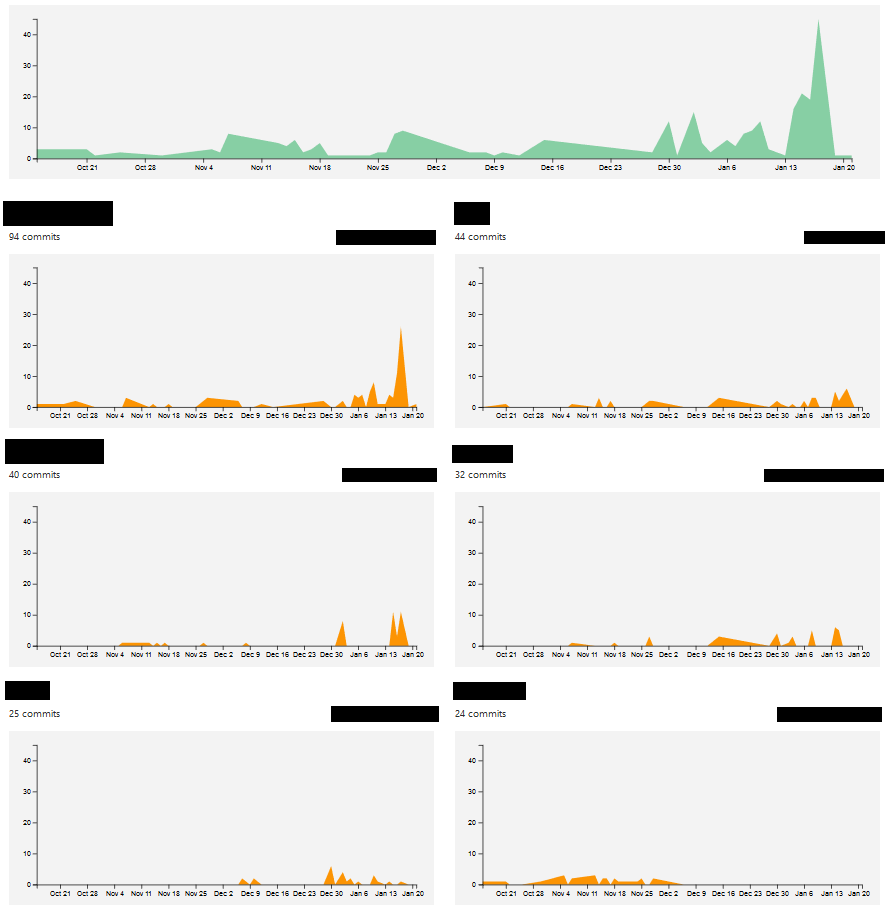
\includegraphics[scale=0.4]{slike/aktivnost.PNG}
			\centering
			\caption{Primjer slike s potpisom}
			\label{fig:promjene}
		\end{figure}
		
		\begin{figure}[H]
			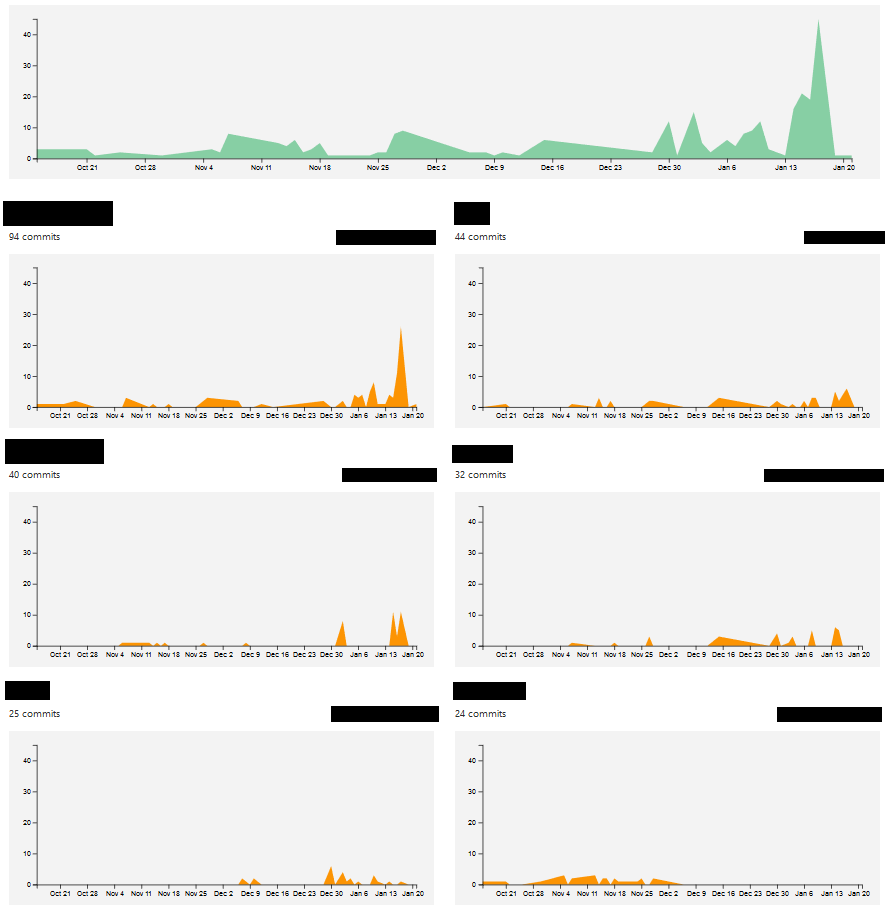
\includegraphics[width=\linewidth]{slike/aktivnost.PNG}
			\caption{Primjer slike s potpisom 2}
			\label{fig:promjene2}
		\end{figure}
		
		
		
		\eject
		
	
	\chapter{Specifikacija programske potpore}
		
	\section{Funkcionalni zahtjevi}
			
			\textbf{\textit{dio 1. revizije}}\\
			
			\textit{Navesti \textbf{dionike} koji imaju \textbf{interes u ovom sustavu} ili  \textbf{su nositelji odgovornosti}. To su prije svega korisnici, ali i administratori sustava, naručitelji, razvojni tim.}\\
				
			\textit{Navesti \textbf{aktore} koji izravno \textbf{koriste} ili \textbf{komuniciraju sa sustavom}. Oni mogu imati inicijatorsku ulogu, tj. započinju određene procese u sustavu ili samo sudioničku ulogu, tj. obavljaju određeni posao. Za svakog aktora navesti funkcionalne zahtjeve koji se na njega odnose.}\\
			
			
			\noindent \textbf{Dionici:}
			
			\begin{packed_enum}
				
				\item Dionik 1
				\item Dionik 2				
				\item ...
				
			\end{packed_enum}
			
			\noindent \textbf{Aktori i njihovi funkcionalni zahtjevi:}
			
			
			\begin{packed_enum}
				\item  \underbar{Aktor 1 (inicijator) može:}
				
				\begin{packed_enum}
					
					\item funkcionalnost 1
					\item funkcionalnost 2
					\begin{packed_enum}
						
						\item  podfunkcionalnost 1 
						\item  podfunkcionalnost 2
				
					\end{packed_enum}
					\item  funkcionalnost 3
					
				\end{packed_enum}
			
				\item  \underbar{Aktor 2 (sudionik) može:}
				
				\begin{packed_enum}
					
					\item funkcionalnost 1
					\item funkcionalnost 2
					
				\end{packed_enum}
			\end{packed_enum}
			
			\eject 
			
			
				
			\subsection{Obrasci uporabe}
				
				\textbf{\textit{dio 1. revizije}}
				
				\subsubsection{Opis obrazaca uporabe}
					\textit{Funkcionalne zahtjeve razraditi u obliku obrazaca uporabe. Svaki obrazac je potrebno razraditi prema donjem predlošku. Ukoliko u nekom koraku može doći do odstupanja, potrebno je to odstupanje opisati i po mogućnosti ponuditi rješenje kojim bi se tijek obrasca vratio na osnovni tijek.}\\
					

					\noindent \underbar{\textbf{UC$<$broj obrasca$>$ -$<$ime obrasca$>$}}
					\begin{packed_item}
	
						\item \textbf{Glavni sudionik: }$<$sudionik$>$
						\item  \textbf{Cilj:} $<$cilj$>$
						\item  \textbf{Sudionici:} $<$sudionici$>$
						\item  \textbf{Preduvjet:} $<$preduvjet$>$
						\item  \textbf{Opis osnovnog tijeka:}
						
						\item[] \begin{packed_enum}
	
							\item $<$opis korak jedan$>$
							\item $<$opis korak dva$>$
							\item $<$opis korak tri$>$
							\item $<$opis korak četiri$>$
							\item $<$opis korak pet$>$
						\end{packed_enum}
						
						\item  \textbf{Opis mogućih odstupanja:}
						
						\item[] \begin{packed_item}
	
							\item[2.a] $<$opis mogućeg scenarija odstupanja u koraku 2$>$
							\item[] \begin{packed_enum}
								
								\item $<$opis rješenja mogućeg scenarija korak 1$>$
								\item $<$opis rješenja mogućeg scenarija korak 2$>$
								
							\end{packed_enum}
							\item[2.b] $<$opis mogućeg scenarija odstupanja u koraku 2$>$
							\item[3.a] $<$opis mogućeg scenarija odstupanja  u koraku 3$>$
							
						\end{packed_item}
					\end{packed_item}
				
					
				\subsubsection{Dijagrami obrazaca uporabe}
					
					\textit{Prikazati odnos aktora i obrazaca uporabe odgovarajućim UML dijagramom. Nije nužno nacrtati sve na jednom dijagramu. Modelirati po razinama apstrakcije i skupovima srodnih funkcionalnosti.}
					
					\begin{figure}[H]
						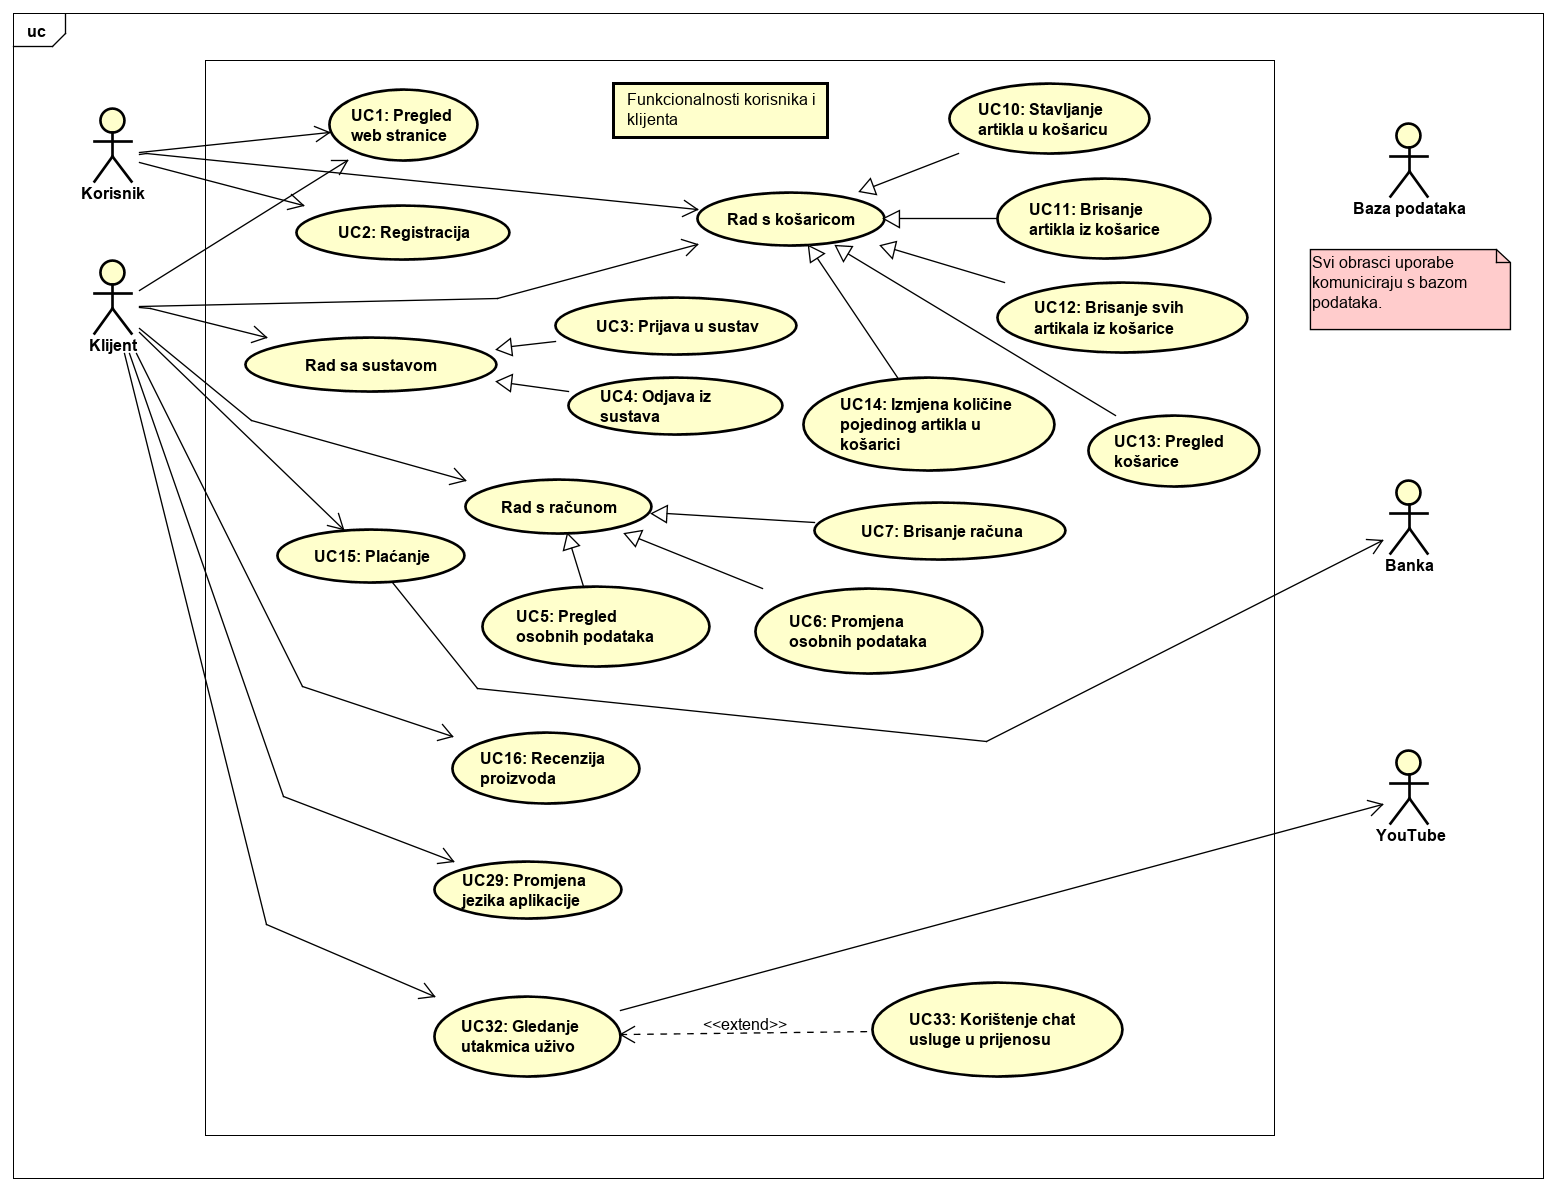
\includegraphics[scale=0.4]{dijagrami/Funkcionalnosti_korisnika_i_klijenta.png}
						\centering
						\caption{Funkcionalnosti korisnika i klijenta}
						\label{fig:UseCaseDiagram1}
					\end{figure}
				
					\begin{figure}[H]
						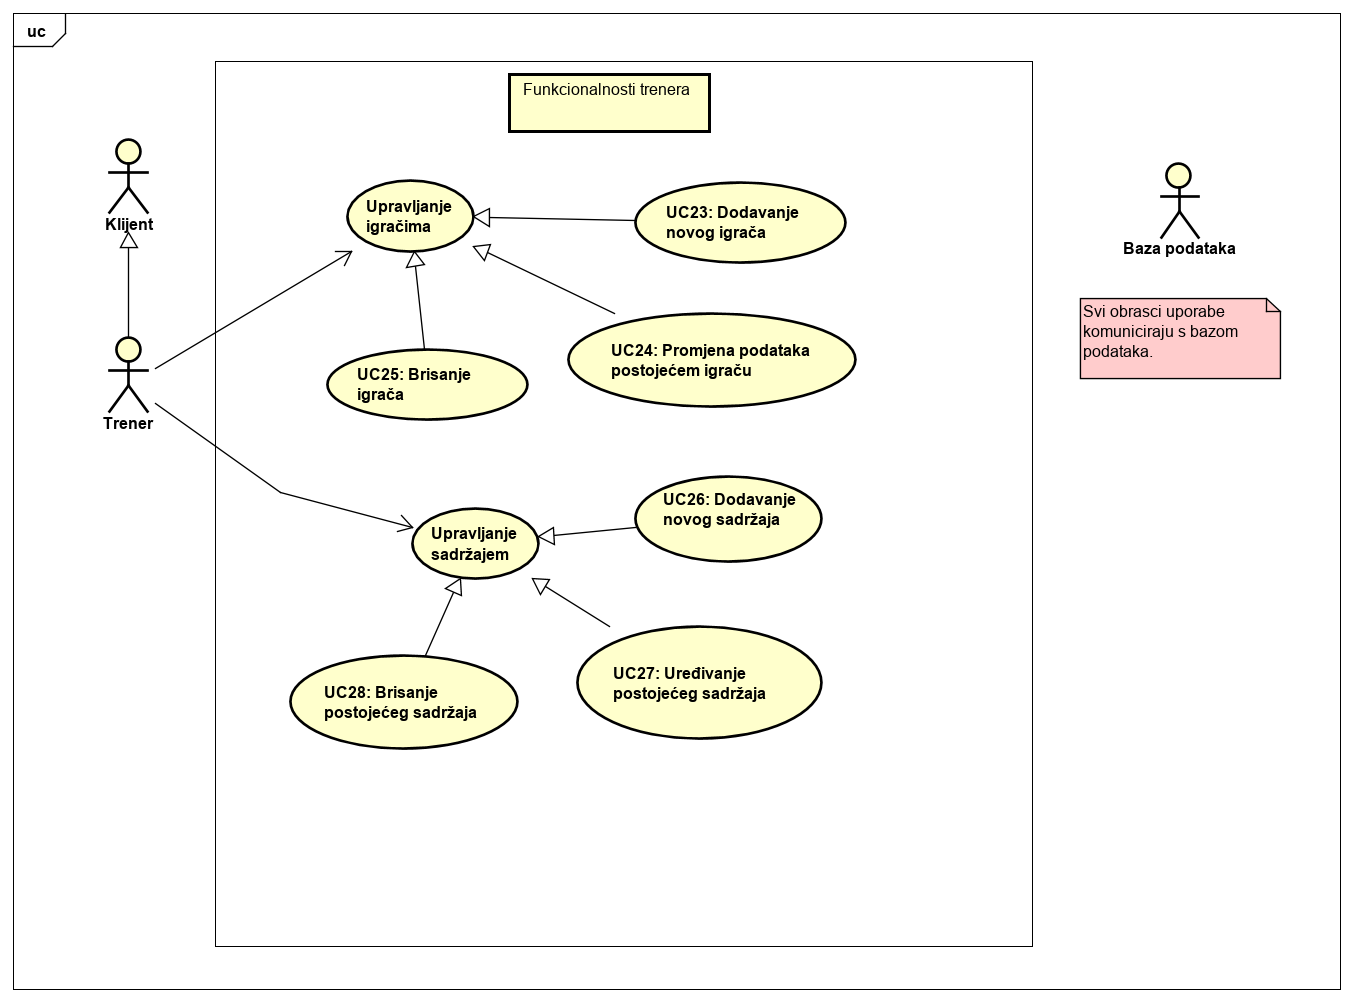
\includegraphics[scale=0.4]{dijagrami/Funkcionalnosti_trenera.png}
						\centering
						\caption{Funkcionalnosti trenera}
						\label{fig:UseCaseDiagram2}
					\end{figure}
				
					\begin{figure}[H]
						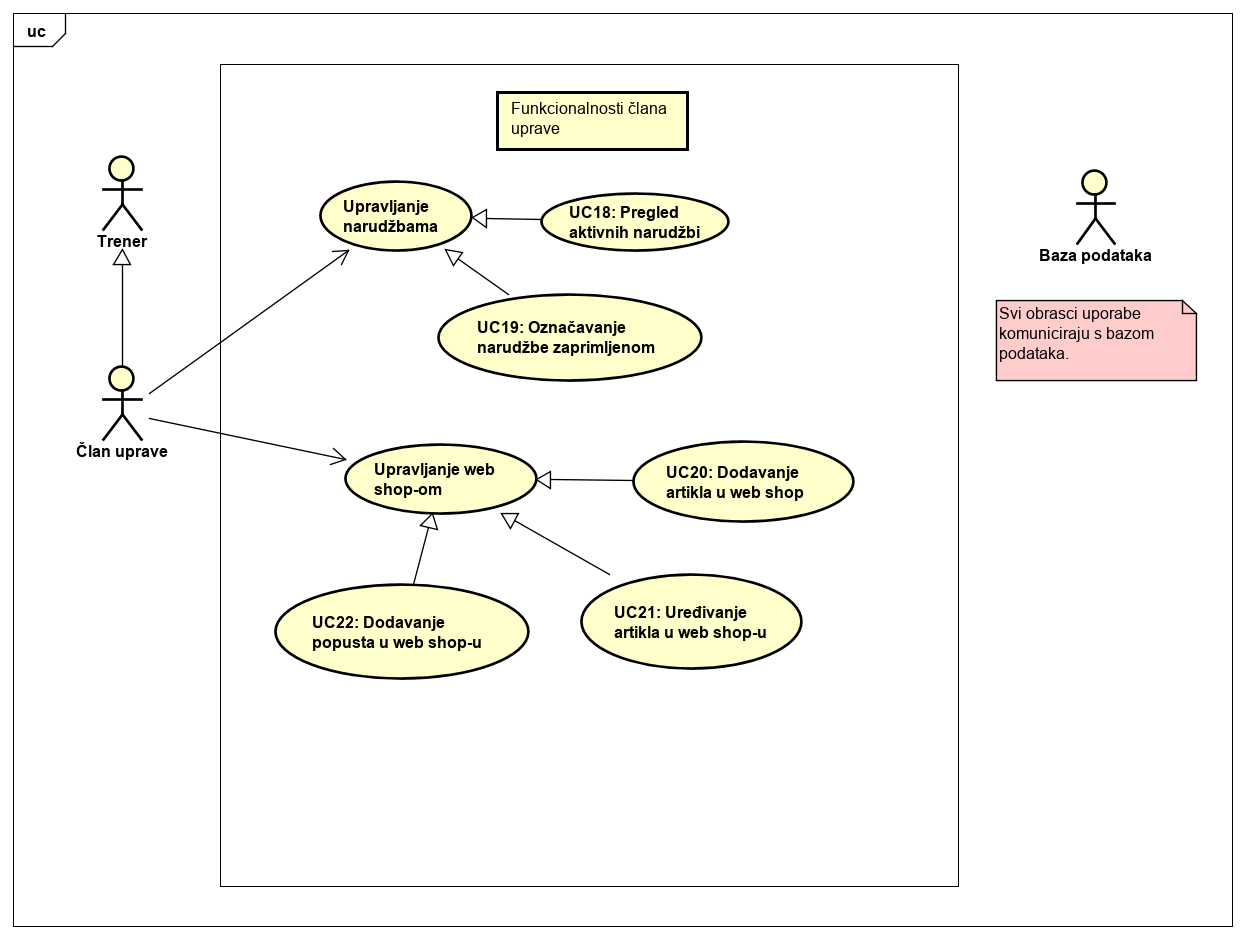
\includegraphics[scale=0.4]{dijagrami/Funkcionalnosti_clana_uprave.png}
						\centering
						\caption{Funkcionalnosti člana uprave}
						\label{fig:UseCaseDiagram3}
					\end{figure}
				
					\begin{figure}[H]
						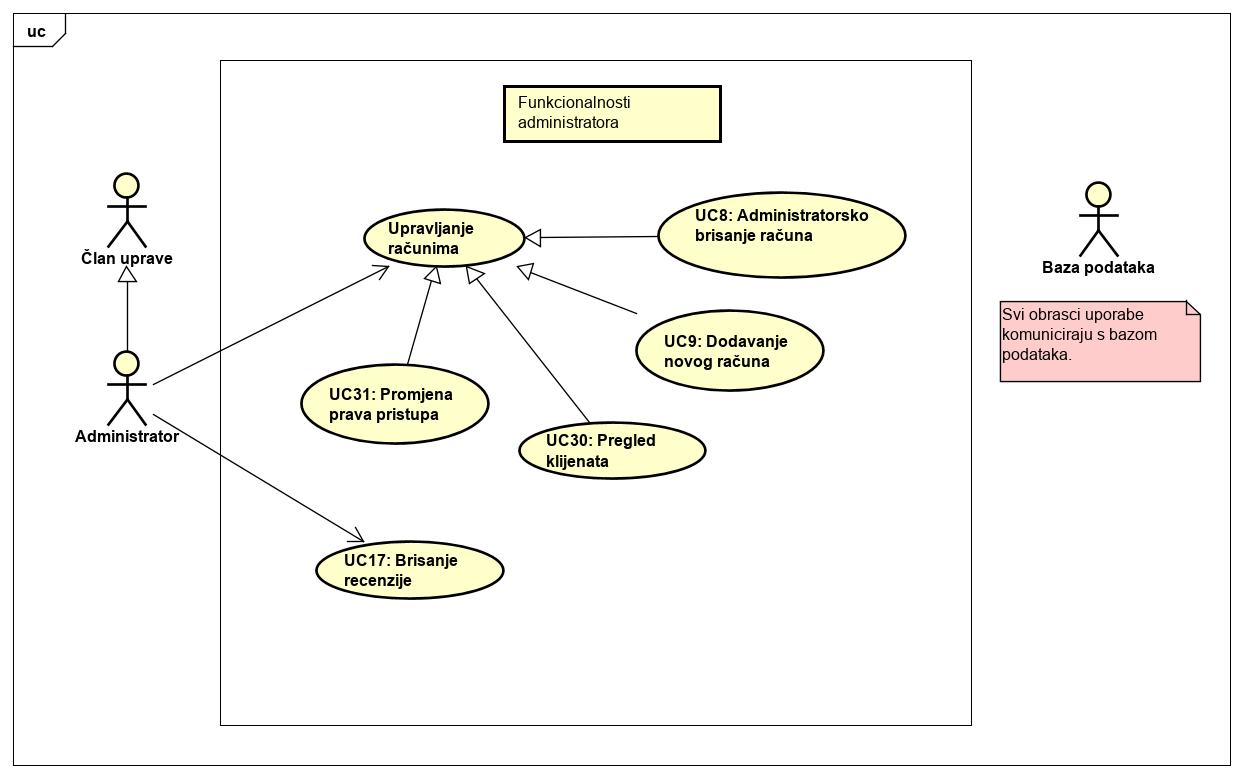
\includegraphics[scale=0.4]{dijagrami/Funkcionalnosti_administratora.png}
						\centering
						\caption{Funkcionalnosti administratora}
						\label{fig:UseCaseDiagram4}
					\end{figure}
				
				\eject		
				
			\subsection{Sekvencijski dijagrami}
				
				\textbf{\textit{dio 1. revizije}}\\
				
				\textit{Nacrtati sekvencijske dijagrame koji modeliraju najvažnije dijelove sustava (max. 4 dijagrama). Ukoliko postoji nedoumica oko odabira, razjasniti s asistentom. Uz svaki dijagram napisati detaljni opis dijagrama.}
				\eject
				
				\begin{figure}[H]
					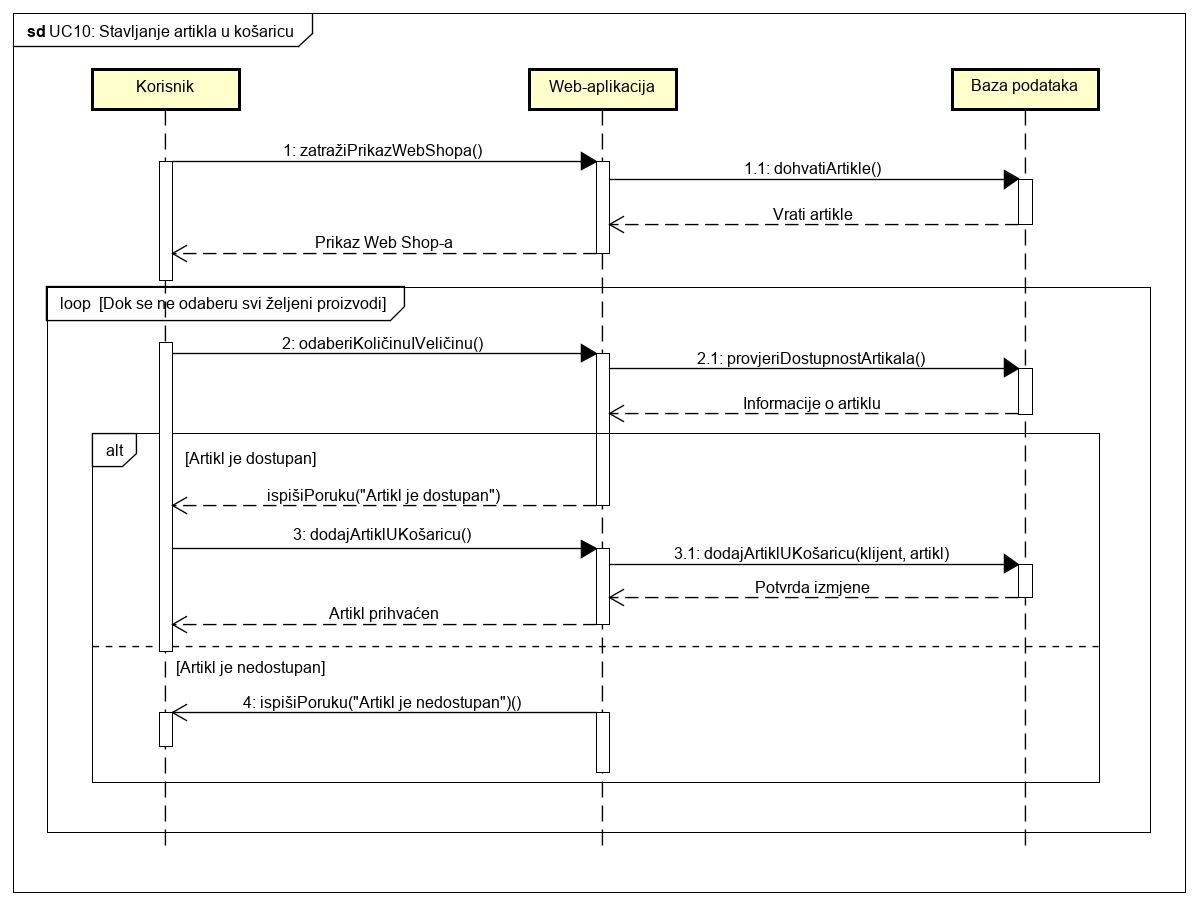
\includegraphics[scale=0.4]{dijagrami/UC10.png}
					\centering
					\caption{UC10, Stavljanje artikla u košaricu}
					\label{fig:SequanceDiagram1}
				\end{figure}
			
				\begin{figure}[H]
					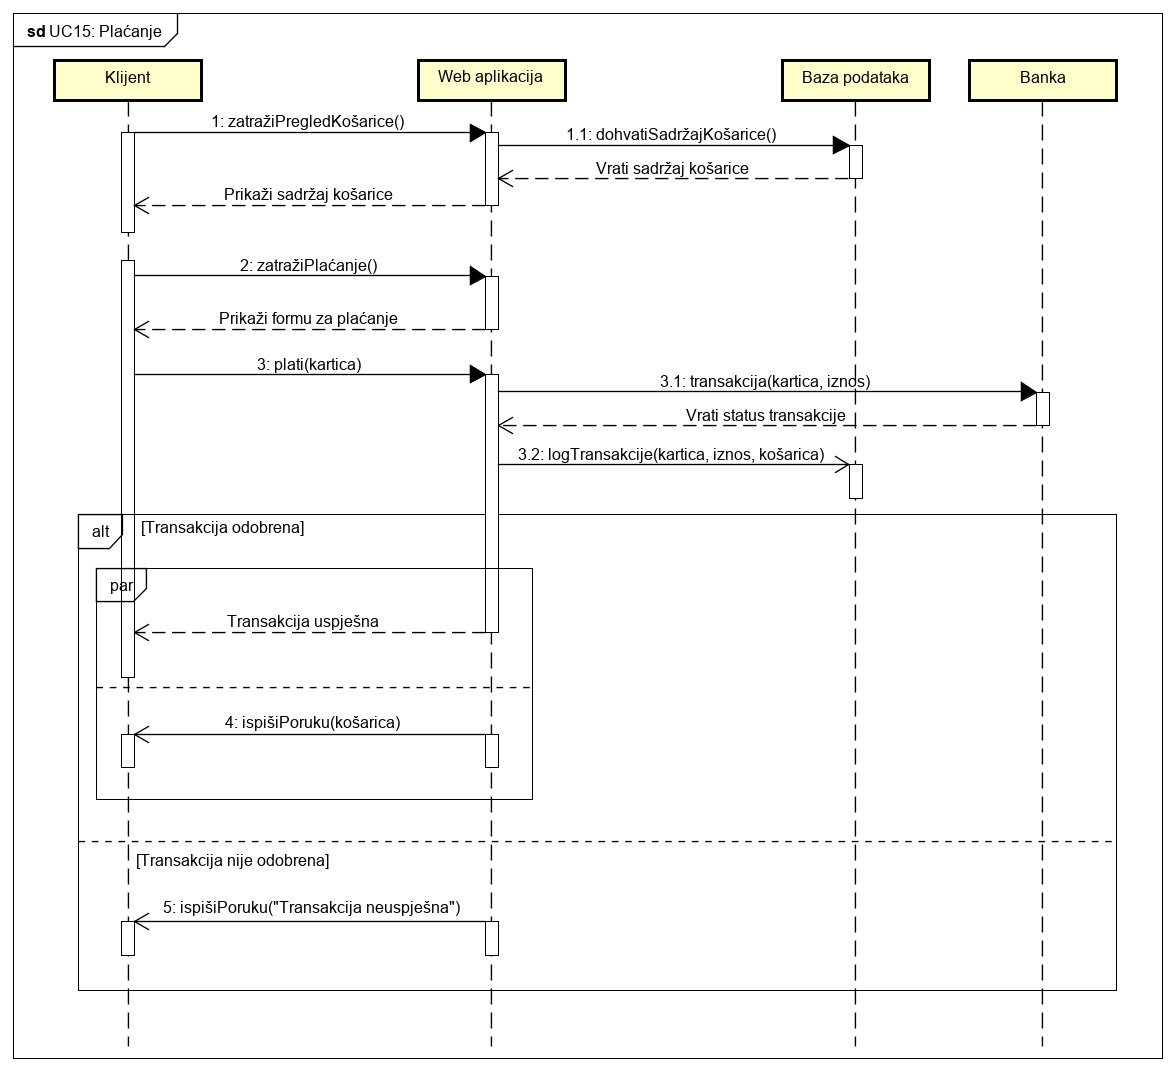
\includegraphics[scale=0.4]{dijagrami/UC15.png}
					\centering
					\caption{UC15, Plaćanje}
					\label{fig:SequanceDiagram2}
				\end{figure}
			
				\begin{figure}[H]
					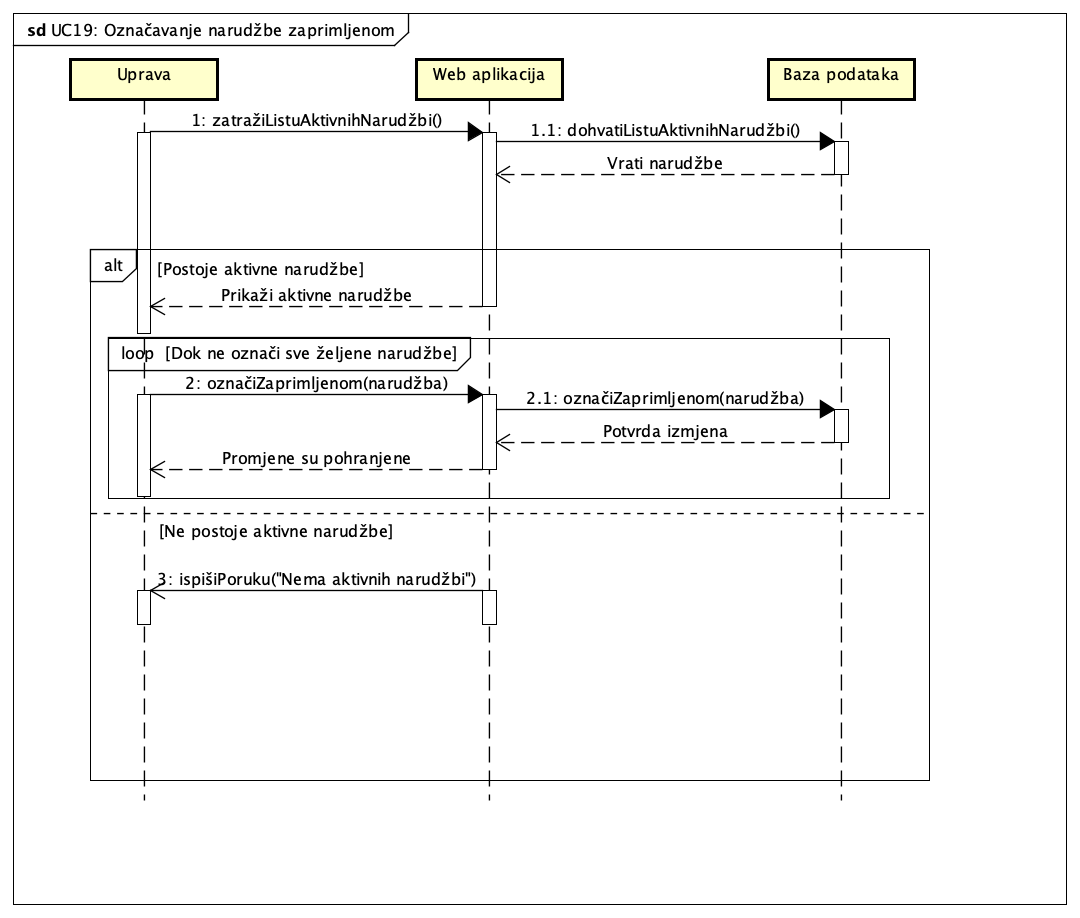
\includegraphics[scale=0.4]{dijagrami/UC19.png}
					\centering
					\caption{UC19, Označavanje narudžbe gotovom}
					\label{fig:SequanceDiagram3}
				\end{figure}
			
				\begin{figure}[H]
					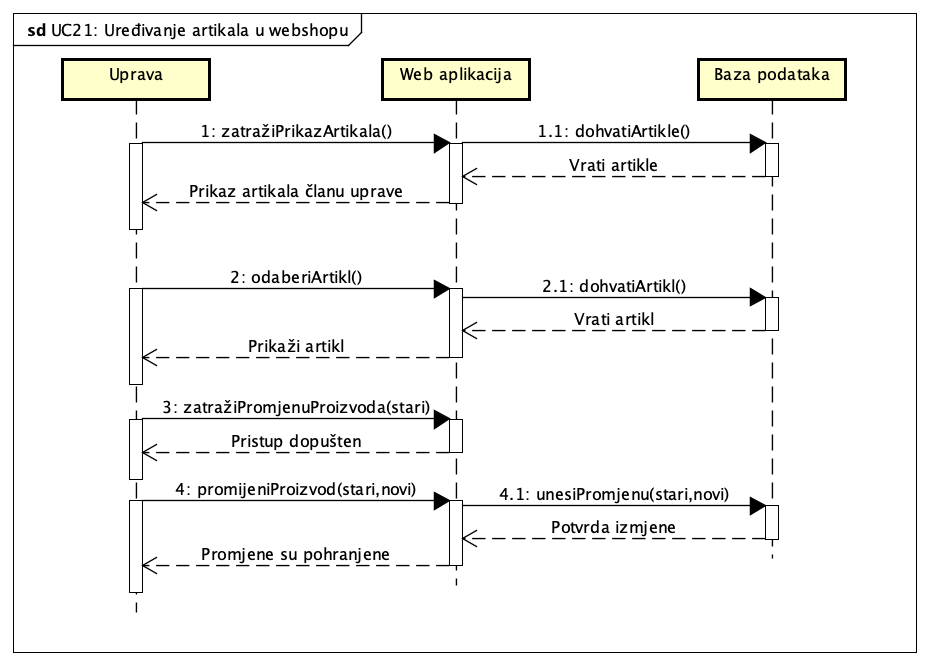
\includegraphics[scale=0.4]{dijagrami/UC21.png}
					\centering
					\caption{UC21, Uređivanje artikala u web shopu}
					\label{fig:SequanceDiagram4}
				\end{figure}
	
		\section{Ostali zahtjevi}
		
			\begin{packed_item}
				\item Sustav treba omogućiti rad više korisnika u stvarnom vremenu
				\item Korisničko sučelje i sustav moraju podržavati hrvatsku abecedu (dijakritičke znakove) pri unosu i prikazu tekstualnog sadržaja
				\item Izvršavanje dijela programa u kojem se pristupa bazi podataka ne smije trajati duže od nekoliko sekundi
				\item Sustav treba biti implementiran kao web aplikacija koristeći objektno-orijentirane jezike
				\item Neispravno korištenje korisničkog sučelja ne smije narušiti funkcionalnost i rad sustava
				\item Sustav treba biti jednostavan za korištenje, korisnici se moraju znati koristiti sučeljem bez opširnih uputa
				\item Nadogradnja sustava ne smije narušavati postojeće funkcionalnosti sustava
				\item Sustav kao valutu koristi HRK
				\item Veza s bazom podataka mora biti kvalitetno zaštićena, brza i otporna na vanjske greške
				\item Front-end web aplikacije bit će implementiran uz pomoć HTML5, CSS3, Bootstrap 4 i Vue.js tehnologija
				\item Back-end web aplikacije bit će implementiran u programskom jeziku C\#
				\item Čitav sustav će biti utemeljen na okviru rada ASP.NET Core 3.0
				\item Sustav će podržavati hrvatski i engleski jezik
			\end{packed_item}

			 
			 
			 
	
	\chapter{Arhitektura i dizajn sustava}
		

		\textnormal{ Arhitektura sustava ovog projekta može se podijeliti u tri dijela:}
	\begin{itemize}
		\item 	\textit{Baza podataka}
		\item 	\textit{Web aplikacija}
		\item 	\textit{Web poslužitelj}		
	\end{itemize}
\textnormal {\textbf{Web poslužitelj} osnova je rada web aplikacije. Njegova primarna zadaća je komunikacija klijenta s aplikacijom. Komunikacija se odvija preko HTTP (engl. Hyper Text Transfer Protocol) protokola. Poslužitelj je onaj koji pokreće web aplikaciju te joj prosljeđuje zahtjev. \textbf{Web preglednik} je program koji korisniku omogućuje pregled web stranica i multimedijalnih sadržaja vezanih uz njih. Korisnik i web aplikacija komuniciraju s web preglednikom. Korisnik preko \textbf{web aplikacije} šalje zahtjeve. Web aplikacija obrađuje zahtjeve te komunicira s bazom podataka. }
\bigbreak
\textnormal {Programski jezik koji smo odabrali za našu web aplikaciju jest C\#. Odabrali smo ga jer je većina današnjih web aplikacija napisana u C\#. Također, odlučili smo se na ASP.NET Core 3 radni okvir koji pruža mnogo funkcionalnosti. Koristimo i Vue.js radni okvir za JavaScript. Za razvojno okruženje odabrali smo Microsoft Visual Studio.}
\bigbreak
\textnormal{Arhitektura sustava temelji se na MVC (Model-View-Controller) konceptu. Taj je koncept podržan od ASP.NET Core 3 radnog okvira i olakšava razvoj web aplikacije zbog svojih gotovih predložaka. MVC koncept karakterističan je po tome što se pojedini dijelovi aplikacije mogu razvijati nezavisno, što uvelike olakšava testiranje, razvijanje te dodavanje novih mogućnosti u sustav. MVC koncept sadržava:}
\bigbreak
	\begin{itemize}
	\item 	\textbf{Model} - prima ulazne podatke od Controllera, predstavlja strukture podataka koje su dinamične i neovisne o korisničkom sučelju. Središnja je komponenta sustava jer izravno upravlja pravilima web aplikacije.
	\item 	\textbf{View} - prikaz podataka s mogućnosću različitih prikaza.
	\item 	\textbf{Controller}	- upravlja korisničkim zahtjevima te prima ulaze i prilagođava ih za prosljeđivanje Modelu ili Viewu, ovisno o potrebi.
\end{itemize}

	
		

		

				
		\section{Baza podataka}
			
			
		\textnormal{Za naš projekt odabrali smo relacijsku bazu podataka. Njezina osnovna jedinica je tablica definirana imenom i skupom atributa. Zadaća naše baze podataka je brza i jednostavna pohrana podataka, izmjena, brisanje i dohvat tih podataka. Baza podataka ove aplikacije sastoji se od sljedećih entiteta:}
		\smallbreak
			\begin{packed_item}
				\setlength\itemsep{0.01em}
			\item  Košarica
			\item  Korisnik
			\item  Narudžba
			\item Transakcija
			\item Artikl košarice
			\item Artikl narudžbe
			\item Artikl
			\item Artikl dostupnost
			\item Recenzija
			\item Utakmica
			\item Popust
			\item Slika
			\item Objava
			\item Igrač
		\end{packed_item}
		
		\pagebreak
		
			\subsection{Opis tablica}
			
				\textnormal{U nastavku su opisane tablice baze podatka. U napisanim tablicama je ključ tablice podebljan, a strani ključevi su napisani kurzivom.}
				
				\bigbreak

				\textnormal{Tablica \textbf{Korisnik} opisuje svakog korisnika, klijenta, trenera, upravu ili administratora aplikacije. Sadrži atribute: korisničko ime, ime, prezime, e-mail, hash lozinke, razinu ovlasti, broj mobitela i datum registracije. Povezana je vezom \textit{One-to-Many} s entitetima Narudžba, Košarica i Recenzija preko korisničkog imena.}
				
				\begin{longtabu} to \textwidth {|X[8, l]|X[6, l]|X[20, l]|}
					
					\hline \multicolumn{3}{|c|}{\textbf{Korisnik}}	 \\[3pt] \hline
					\endfirsthead
					
					\hline \multicolumn{3}{|c|}{\textbf{Korisnik}}	 \\[3pt] \hline
					\endhead
					
					\hline 
					\endlastfoot
					
					\textbf{korisnicko\_ime}  & VARCHAR	&  jedinstveni identifikator korisnika	\\ \hline
					ime	& VARCHAR &   ime korisnika	\\ \hline 
					prezime & VARCHAR & prezime korisnika \\ \hline
					e-mail & VARCHAR & e-mail korisnika  \\ \hline 
					lozinka\_hash & VARCHAR	&  	hash lozinke	\\ \hline 
					razina\_ovlasti & INT & razina ovlasti korisnika \\ \hline
					broj\_mob & VARCHAR & broj mobitela korisnika \\ \hline 
					datum\_registracije	& TIMESTAMP & datum registracije korisnika   	\\ \hline 
					
					
				\end{longtabu}
			
			\textnormal{Tablica \textbf{Košarica} opisuje košarice koje se koriste u web shop-u. Sadrži atribute: ID, korisničko ime te datum kreiranja košarice. Povezana je vezom \textit{One-to-Many} s entitetom Artikl Košarice preko ID-a i \textit{Many-to-One} s entitetom Korisnik preko korisničkog imena. }
			
			\begin{longtabu} to \textwidth {|X[8, l]|X[6, l]|X[20, l]|}
				
				\hline \multicolumn{3}{|c|}{\textbf{Košarica}}	 \\[3pt] \hline
				\endfirsthead
				
				\hline \multicolumn{3}{|c|}{\textbf{Košarica }}	 \\[3pt] \hline
				\endhead
				
				\hline 
				\endlastfoot
				
				\textbf{ID} & INT	&  jedinstveni identifikator košarice	\\ \hline
				\textit{korisnicko\_ime} 	& VARCHAR &   ime korisnika koji koristi košaricu	\\ \hline 
				datum& TIMESTAMP & datum kreiranja košarice	\\ \hline 
				
			\end{longtabu}
		
		
		\textnormal{Tablica \textbf{Artikl Košarice} opisuje artikle košarice koje se koriste u web shop-u. Sadrži atribute: ID košarice, ID artikla, količinu artikla, veličinu artikla, kupovnu cijenu i kupovni popust. Povezana je vezom \textit{Many-to-One} s entitetima Artikl i Košarica preko ID artikla, odnosno ID košarice.}
		
		\begin{longtabu} to \textwidth {|X[8, l]|X[6, l]|X[20, l]|}
			
			\hline \multicolumn{3}{|c|}{\textbf{Artikl Košarice}}	 \\[3pt] \hline
			\endfirsthead
			
			\hline \multicolumn{3}{|c|}{\textbf{Artikl Košarice }}	 \\[3pt] \hline
			\endhead
			
			\hline 
			\endlastfoot
			
			\textbf{ID\_košarice} & INT	&  jedinstveni identifikator košarice	\\ \hline
			\textbf{ID\_artikla}	& int &  jedinstveni identifikator artikla	\\ \hline 
			kolicina & INT  & količina artikla \\ \hline 
			velicina & VARCHAR  & veličina artikla \\ \hline 
			kupovna\_cijena & DECIMAL  & kupovna cijena artikla \\ \hline 
			kupovni\_popust & INT  & kupovni popust artikla  \\ \hline 
			
		\end{longtabu}
		\textnormal{Tablica \textbf{Recenzija} opisuje recenzije ostavljene artiklu u web shop-u. Sadrži atribute: ID, ID artikla, datum, ocjena, komentar, korisničko ime i blokirano. Povezana je vezom \textit{Many-to-One} s entitima Artikl i Korisnik preko ID artikla, odnosno korisničkog imena. }
	
	\begin{longtabu} to \textwidth {|X[8, l]|X[6, l]|X[20, l]|}
		
		\hline \multicolumn{3}{|c|}{\textbf{Recenzija}}	 \\[3pt] \hline
		\endfirsthead
		
		\hline \multicolumn{3}{|c|}{\textbf{Recenzija}}	 \\[3pt] \hline
		\endhead
		
		\hline 
		\endlastfoot
		
		\textbf{ID} & INT	&  jedinstveni identifikator recenzije	\\ \hline
		\textit{ID\_artikla}	& INT &  jedinstveni identifikator artikla	\\ \hline 
		datum & TIMESTAMP  & datum dodavanja recenzije \\ \hline 
		ocjena & INT  & ocjena artikla \\ \hline 
		komentar & VARCHAR  & komentar recenzije \\ \hline 
		korisnicko\_ime & INT  & korisničko ime korisnika koji ostavlja recenziju  \\ \hline 
		blokirano & BOOLEAN  & dozvoljena ili blokirana recenzija \\ \hline 
		
	\end{longtabu}

	\textnormal{Tablica \textbf{Utakmica} opisuje utakmice kluba. Sadrži atribute: ID, datum, tim domacin, tim gost, mjesto, dvorana i drzava. }

\begin{longtabu} to \textwidth {|X[8, l]|X[6, l]|X[20, l]|}
	
	\hline \multicolumn{3}{|c|}{\textbf{Utakmica}}	 \\[3pt] \hline
	\endfirsthead
	
	\hline \multicolumn{3}{|c|}{\textbf{Utakmica}}	 \\[3pt] \hline
	\endhead
	
	\hline 
	\endlastfoot
	
	\textbf{ID} & INT	&  jedinstveni identifikator utakmice	\\ \hline
	datum & TIMESTAMP &  jedinstveni identifikator artikla	\\ \hline 
	tim\_domacin & VARCHAR  & tim domaćin utakmice \\ \hline 
	tim\_gost & VARCHAR  & tim gost utakmice  \\ \hline 
	mjesto & VARCHAR  & mjesto održavanja utakmice \\ \hline 
	dvorana & VARCHAR  & dvorana održavanja utakmice \\ \hline 
	drzava & VARCHAR  & država održavanja utakmice \\ \hline 
	
\end{longtabu}

\textnormal{Tablica \textbf{Popust} opisuje popuste na artikl dodane na web shop. Sadrži atribute: ID, ID artikla, datum, datum pocetka, datum kraja i postotak popusta. Entitet je povezan vezom \textit{Many-to-One} s entitetom Artikl preko ID artikla.}

\begin{longtabu} to \textwidth {|X[8, l]|X[6, l]|X[20, l]|}
	
	\hline \multicolumn{3}{|c|}{\textbf{Popust}}	 \\[3pt] \hline
	\endfirsthead
	
	\hline \multicolumn{3}{|c|}{\textbf{Popust}}	 \\[3pt] \hline
	\endhead
	
	\hline 
	\endlastfoot
	
	\textbf{ID} & INT	&  jedinstveni identifikator popusta	\\ \hline
	\textit{ID\_artikla} & INT &  jedinstveni identifikator artikla	\\ \hline 
	datum & TIMESTAMP  & datum stvaranja popusta \\ \hline 
	datum\_pocetka & TIMESTAMP  & datum početka popusta  \\ \hline 
	datum\_kraja & TIMESTAMP  & datum završetka popusta \\ \hline 
	postotak & INT  & postotak popusta \\ \hline 
	
\end{longtabu}

\textnormal{Tablica \textbf{Slika} opisuje slike dodane na web stranicu. Sadrži atribute: ID, path, datum. Entitet je povezan vezom \textit{One-to-Many} s entitetima Artikl, Objava i Igrač preko ID slike.}

\begin{longtabu} to \textwidth {|X[8, l]|X[6, l]|X[20, l]|}
	
	\hline \multicolumn{3}{|c|}{\textbf{Slika}}	 \\[3pt] \hline
	\endfirsthead
	
	\hline \multicolumn{3}{|c|}{\textbf{Slika}}	 \\[3pt] \hline
	\endhead
	
	\hline 
	\endlastfoot
	
	\textbf{ID} & INT	&  jedinstveni identifikator slike	\\ \hline
     path & VARCHAR  &  put do slike	\\ \hline 
	datum & TIMESTAMP  & datum dodavanja slike \\ \hline 
\end{longtabu}

\textnormal{Tablica \textbf{Artikl} opisuje artikle dodane na web shop. Sadrži atribute: ID, datum dodavanja, datum posljednje izmjene, tip, cijenu, naziv, opis, ID slike. Entitet je povezan vezom \textit{One-to-Many} s entitetima Artikl Dostupnost, Popust, Artikl Narudžbe, Recenzija te Artikl Košarice preko ID artikla i vezom \textit{Many-to-One} s entitetom Slika preko ID slike.}

\begin{longtabu} to \textwidth {|X[8, l]|X[6, l]|X[20, l]|}
	
	\hline \multicolumn{3}{|c|}{\textbf{Artikl}}	 \\[3pt] \hline
	\endfirsthead
	
	\hline \multicolumn{3}{|c|}{\textbf{Artikl}}	 \\[3pt] \hline
	\endhead
	
	\hline 
	\endlastfoot
	
	\textbf{ID} & INT	&  jedinstveni identifikator artikla	\\ \hline
	datum\_dodavanja & TIMESTAMP  & datum dodavanja artikla \\ \hline 
	datum\_izmjene & TIMESTAMP  & datum posljednje izmjene slike \\ \hline 
	tip & VARCHAR  & tip artikla \\ \hline 
	cijena & INT  & cijena artikla \\ \hline 
	naziv  & VARCHAR  & naziv artikla \\ \hline 
	opis & VARCHAR  & opis artikla \\ \hline 
	\textit{ID\_slike} & INT  & jedinstveni identifikator slike  \\ \hline 
	 
\end{longtabu}
\textnormal{Tablica \textbf{Narudžba} opisuje narudžbe artikala aplikacije. Sadrži atribute: ID,korisničko ime, datum, zaprimljenost, adresa, mjesto, poštanski broj. Entitet je povezan vezom \textit{One-to-Many} s entitetima Artikl Narudžbe preko ID narudžbe i vezom \textit{Many-to-One} s entitetom Korisnik preko korisničkog imena.}

\begin{longtabu} to \textwidth {|X[8, l]|X[6, l]|X[20, l]|}
	
	\hline \multicolumn{3}{|c|}{\textbf{Narudžba}}	 \\[3pt] \hline
	\endfirsthead
	
	\hline \multicolumn{3}{|c|}{\textbf{Narudžba}}	 \\[3pt] \hline
	\endhead
	
	\hline 
	\endlastfoot
	
	\textbf{ID} & INT	&  jedinstveni identifikator narudžbe	\\ \hline
	\textit{korisnicko\_ime} & VARCHAR  & korisničko ime korisnika koji naručuje \\ \hline 
	datum & TIMESTAMP  & datum formiranja narudžbe\\ \hline 
	zaprimljenost & BOOLEAN  & oznaka zaprimljenosti narudžbe \\ \hline 
	adresa  & VARCHAR  & adresa korisnika koji naručuje \\ \hline 
	mjesto & VARCHAR  & mjesto korisnika koji naručuje\\ \hline 
	postanski\_broj & INT  & poštanski broj korisnika koji naručuje\\ \hline 
	
\end{longtabu}

\textnormal{Tablica \textbf{Objava} opisuje sadržaje objavljene na stranici. Sadrži atribute: ID, naslov, sadržaj, ID slike, datum objave, datum izmjene, vrsta objave, datum pocetka i datum isteka. Entitet je povezan  vezom \textit{Many-to-One} s entitetom Slika preko ID slike.}

\begin{longtabu} to \textwidth {|X[8, l]|X[6, l]|X[20, l]|}
	
	\hline \multicolumn{3}{|c|}{\textbf{Objava}}	 \\[3pt] \hline
	\endfirsthead
	
	\hline \multicolumn{3}{|c|}{\textbf{Objava}}	 \\[3pt] \hline
	\endhead
	
	\hline 
	\endlastfoot
	
	\textbf{ID} & INT	&  jedinstveni identifikator objave	\\ \hline
	 sadržaj & VARCHAR  & sadržaj objave \\ \hline 
	 naslov & VARCHAR  & naslov objave \\ \hline
	\textit{ID\_slike} & ID  & jedinstveni identifikator slike  \\ \hline 
	datum\_objave & TIMESTAMP  & datum postavljanja objave \\ \hline 
	datum\_izmjene & TIMESTAMP  & datum posljednje izmjene objave \\ \hline
	vrsta\_objave & VARCHAR  & vrsta objave \\ \hline 
	datum\_pocetka & TIMESTAMP  & datum početka objave \\ \hline
	datum\_isteka & TIMESTAMP  & datum isteka objave \\ \hline
	
\end{longtabu}
\textnormal{Tablica \textbf{Transakcija} opisuje sve obavljane transakcije. Sadrži atribute: ID, datum, iznos, kartica. Entitet je povezan  vezom \textit{One-to-Many} s entitetom Narudžba preko ID transakcije.}

\begin{longtabu} to \textwidth {|X[8, l]|X[6, l]|X[20, l]|}
	
	\hline \multicolumn{3}{|c|}{\textbf{Transakcija}}	 \\[3pt] \hline
	\endfirsthead
	
	\hline \multicolumn{3}{|c|}{\textbf{Transakcija}}	 \\[3pt] \hline
	\endhead
	
	\hline 
	\endlastfoot
	
	\textbf{ID} & INT	&  jedinstveni identifikator transakcije	\\ \hline
	datum & TIMESTAMP  & datum obavljanja transakcije  \\ \hline 
	iznos & DECIMAL  & iznos transakcije \\ \hline
	kartica & VARCHAR  & kartica transakcije  \\ \hline 
	
\end{longtabu}

\textnormal{Tablica \textbf{Artikl dostupnost} opisuje dostupnost artikala. Sadrži atribute: ID artikla, veličina i količina. Entitet je povezan  vezom \textit{Many-to-One} s entitetom Artikla preko ID artikla.}

\begin{longtabu} to \textwidth {|X[8, l]|X[6, l]|X[20, l]|}
	
	\hline \multicolumn{3}{|c|}{\textbf{Artikl dostupnost}}	 \\[3pt] \hline
	\endfirsthead
	
	\hline \multicolumn{3}{|c|}{\textbf{Artikl dostupnost}}	 \\[3pt] \hline
	\endhead
	
	\hline 
	\endlastfoot
	
	\textbf{ID\_artikla} & INT	&  jedinstveni identifikator artikla	\\ \hline
	\textbf {veličina} & VARCHAR  & veličina artikla \\ \hline
	količina & INT  & količina artikla  \\ \hline 
	
\end{longtabu}

\textnormal{Tablica \textbf{Artikl narudžbe} opisuje sve artikle narudžbe. Sadrži atribute: ID narudžbe, ID artikla, količina, veličina, kupovna cijena i kupovni popust. Entitet je povezan  vezom \textit{Many-to-One} s entitetima Narudžba preko ID narudžbe i Artikl preko ID artikla.}

\begin{longtabu} to \textwidth {|X[8, l]|X[6, l]|X[20, l]|}
	
	\hline \multicolumn{3}{|c|}{\textbf{Artikl narudžbe}}	 \\[3pt] \hline
	\endfirsthead
	
	\hline \multicolumn{3}{|c|}{\textbf{Artikl narudžbe}}	 \\[3pt] \hline
	\endhead
	
	\hline 
	\endlastfoot
	
	\textbf{ID\_narudzbe} & INT	&  jedinstveni identifikator narudžbe	\\ \hline
	\textbf{ID\_artikla} & INT	&  jedinstveni identifikator artikla	\\ \hline
	količina & INT  & količina artikla  \\ \hline 
	veličina & VARCHAR  & veličina artikla \\ \hline
	kupovna\_cijena & DECIMAL  & kupovna cijena  \\ \hline 
	kupovni\_popust & INT  & kupovni popust \\ \hline
	
\end{longtabu}

\textnormal{Tablica \textbf{Igrač} opisuje sve igrače. Sadrži atribute: ID, datum dodavanja, datum posljednje izmjene, ime, prezime, ID slike, datum rođenja i pozicija. Entitet je povezan vezom \textit{Many-to-One} s entitetom Slika.}

\begin{longtabu} to \textwidth {|X[8, l]|X[6, l]|X[20, l]|}
	
	\hline \multicolumn{3}{|c|}{\textbf{Igrač}}	 \\[3pt] \hline
	\endfirsthead
	
	\hline \multicolumn{3}{|c|}{\textbf{Igrač}}	 \\[3pt] \hline
	\endhead
	
	\hline 
	\endlastfoot
	
	\textbf{ID\_narudzbe} & INT	&  jedinstveni identifikator igrača	\\ \hline
	datum\_dodavanja & TIMESTAMP  & datum dodavanja igrača \\ \hline 
	datum\_izmjene & TIMESTAMP  & datum izmjene igrača \\ \hline 
	ime & VARCHAR  & ime igrača \\ \hline
	prezime & VARCHAR  & prezime igrača \\ \hline
	\textit{ID\_slike} & INT  & jedinstveni identifikator slike igrača \\ \hline
	datum\_rodenja & DATE  & datum rođenja igrača \\ \hline 
	pozicija & VARCHAR  & pozicija igrača \\ \hline
	
	
\end{longtabu}
	

	
	
		
		
			
			
			\subsection{Dijagram baze podataka}
					\begin{figure}[H]
					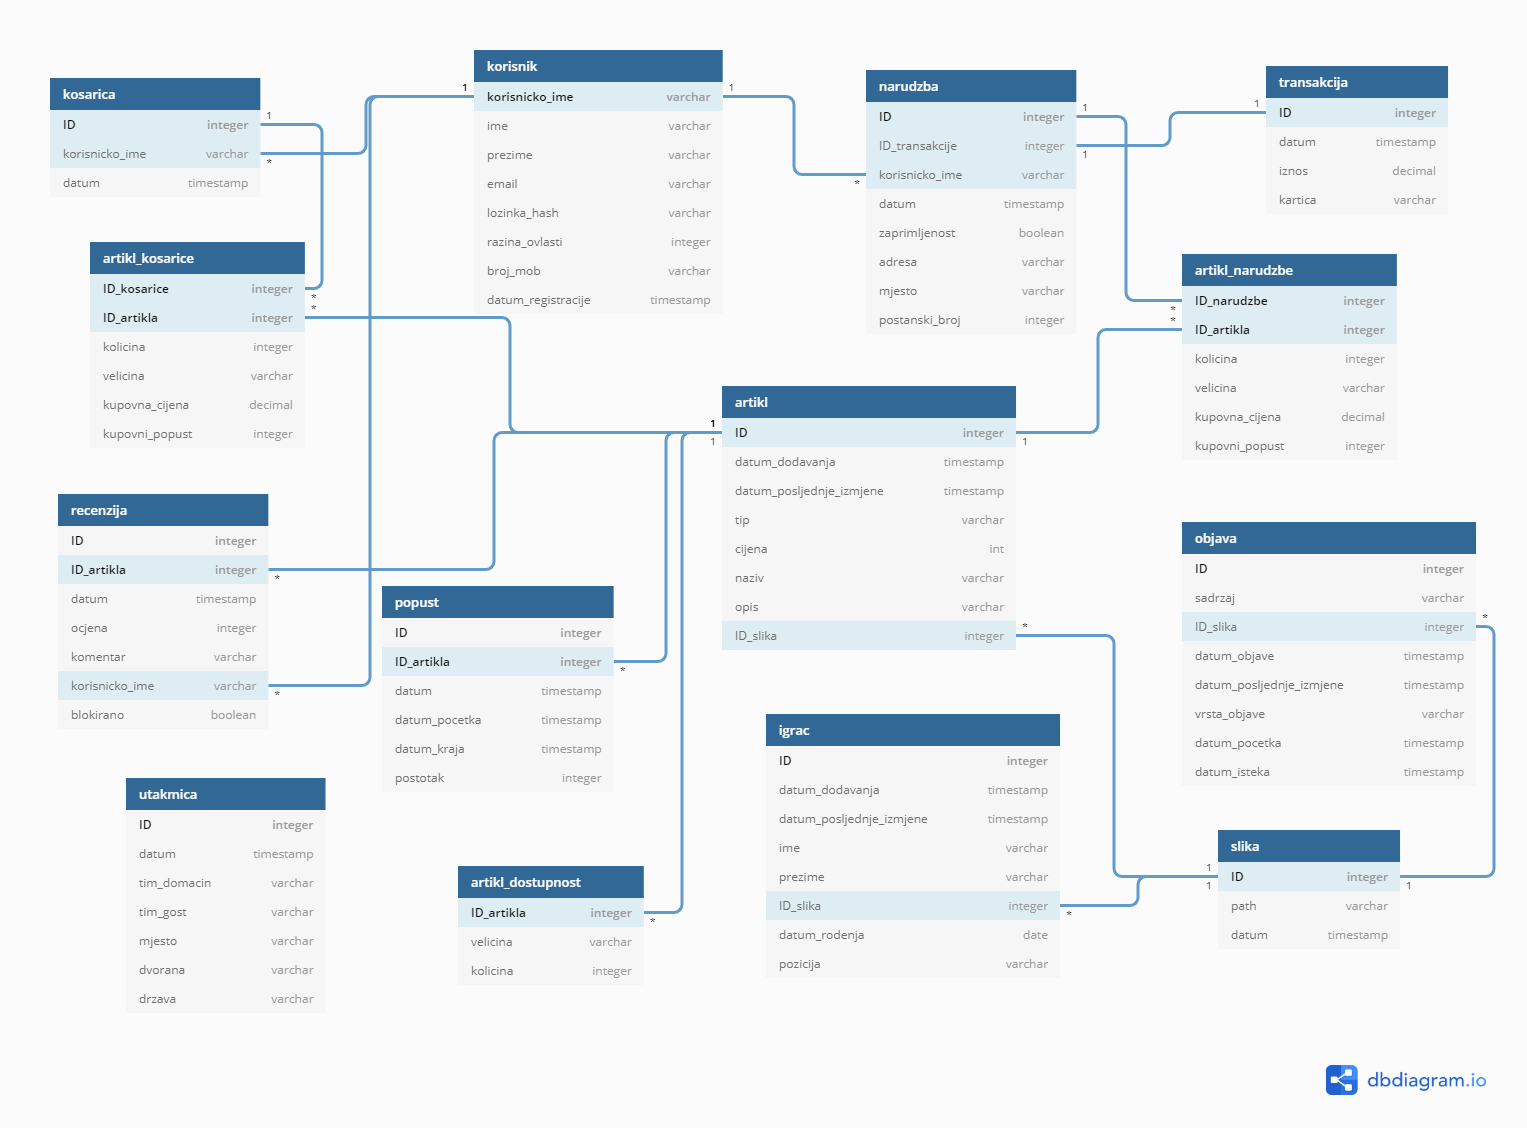
\includegraphics[width=\linewidth]{dijagrami/bazapodataka.png}
					\centering
					\caption{Dijagram baze podataka}
					\label{fig:DatabaseDiagram}
				\end{figure}
			
			\eject
			
			
		\section{Dijagram razreda}
		
			\textnormal{Na slikama 4.2 i 4.3 su prikazani razredi koji pripadaju backend dijelu MVC arhitekture. Razredi prikazani na slici 4.2 nasljeđuju Controller razred. Razredi su podijeljeni prema pravu pristupa metodama određenih aktora. Iz naziva i tipova atributa u razredima može se zaključiti vrsta ovisnosti medu različitim razredima.}\\
			
			\begin{figure}[H]
				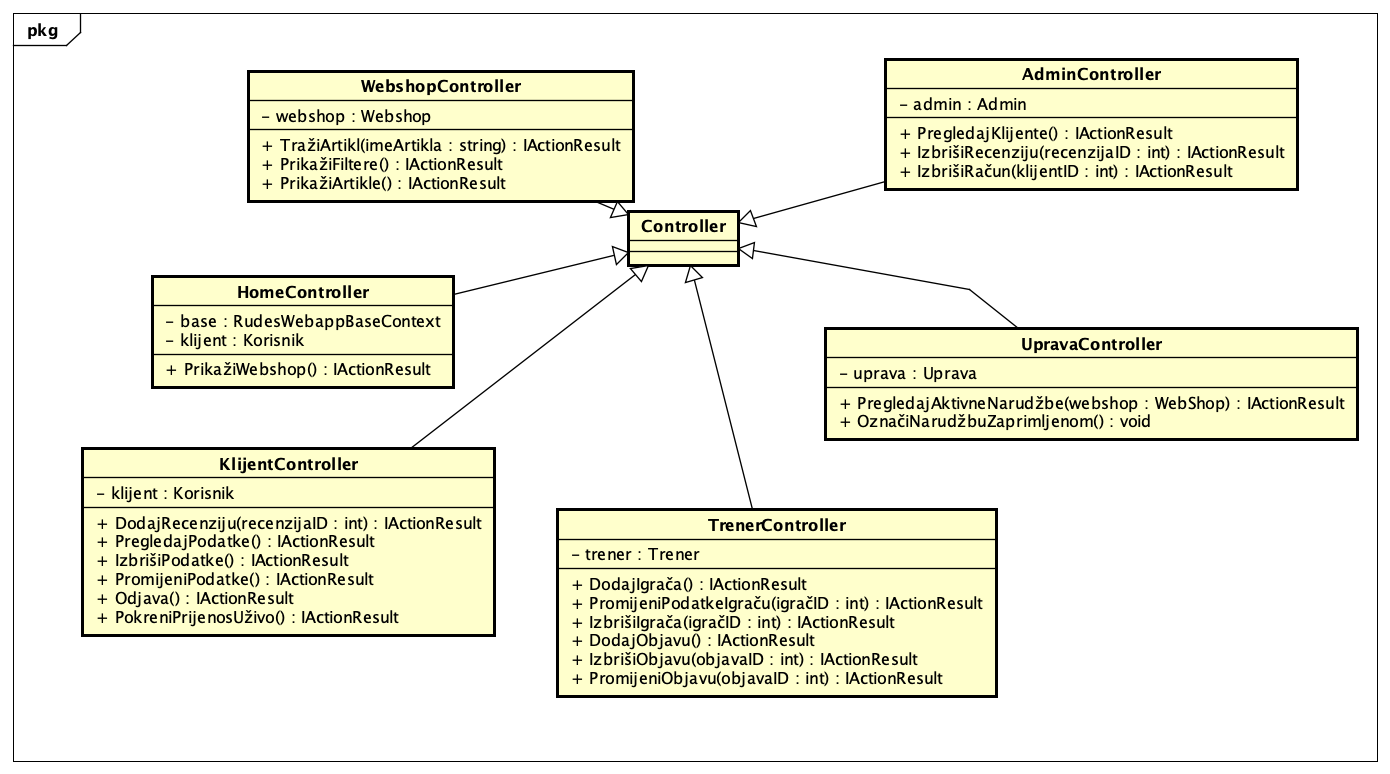
\includegraphics[width=\linewidth]{dijagrami/DijagramRazredaController.png}
				\centering
				\caption{Dijagram razreda - dio Controllers}
				\label{fig:ClassDiagram1}
			\end{figure}
		
			\textnormal{Model razredi na slici 4.3 preslikavaju strukturu baze podataka u aplikaciji. Implementirane metode direktno komuniciraju s bazom podataka te vraćaju tražene podatke. Razred Objava predstavlja objavu bilo koje vrste koja se prikazuje na stranici. Razred Igrač predstavlja igrače kluba kojima se mogu mijenjati podaci. Razred Slika predstavlja sve slike iz objava ili igrača. Razred Utakmica predstavlja utakmice koje klub igra. Nadalje, razredi Artikl, Popust, Artikl Dostupnost i Artikl Košarica predstavljaju artikle, odnosno popuste, dostupnost artikala i artikle stavljene u košaricu web shop-a kluba. Također, razredi Narudžba i Narudžba Artikl i Košarica također su vezani uz web shop. Narudžba predstavlja sve narudžbe korisnika, Narudžba Artikl sve artikle jedne narudžbe, dok razred Košarica predstavlja košaricu web shop-a. Razred Transakcija su sve transakcije koje se obavljaju u web shop-u između klijenata kluba i banke. Razred Recenzija predstavlja recenzije proizvoda u web shopu koje razred Korisnik može ostaviti. Razred Korisnik predstavlja korisnike sustava koji se mogu registrirati i prijaviti u sustav.}\\
		
		\begin{figure}[H]
			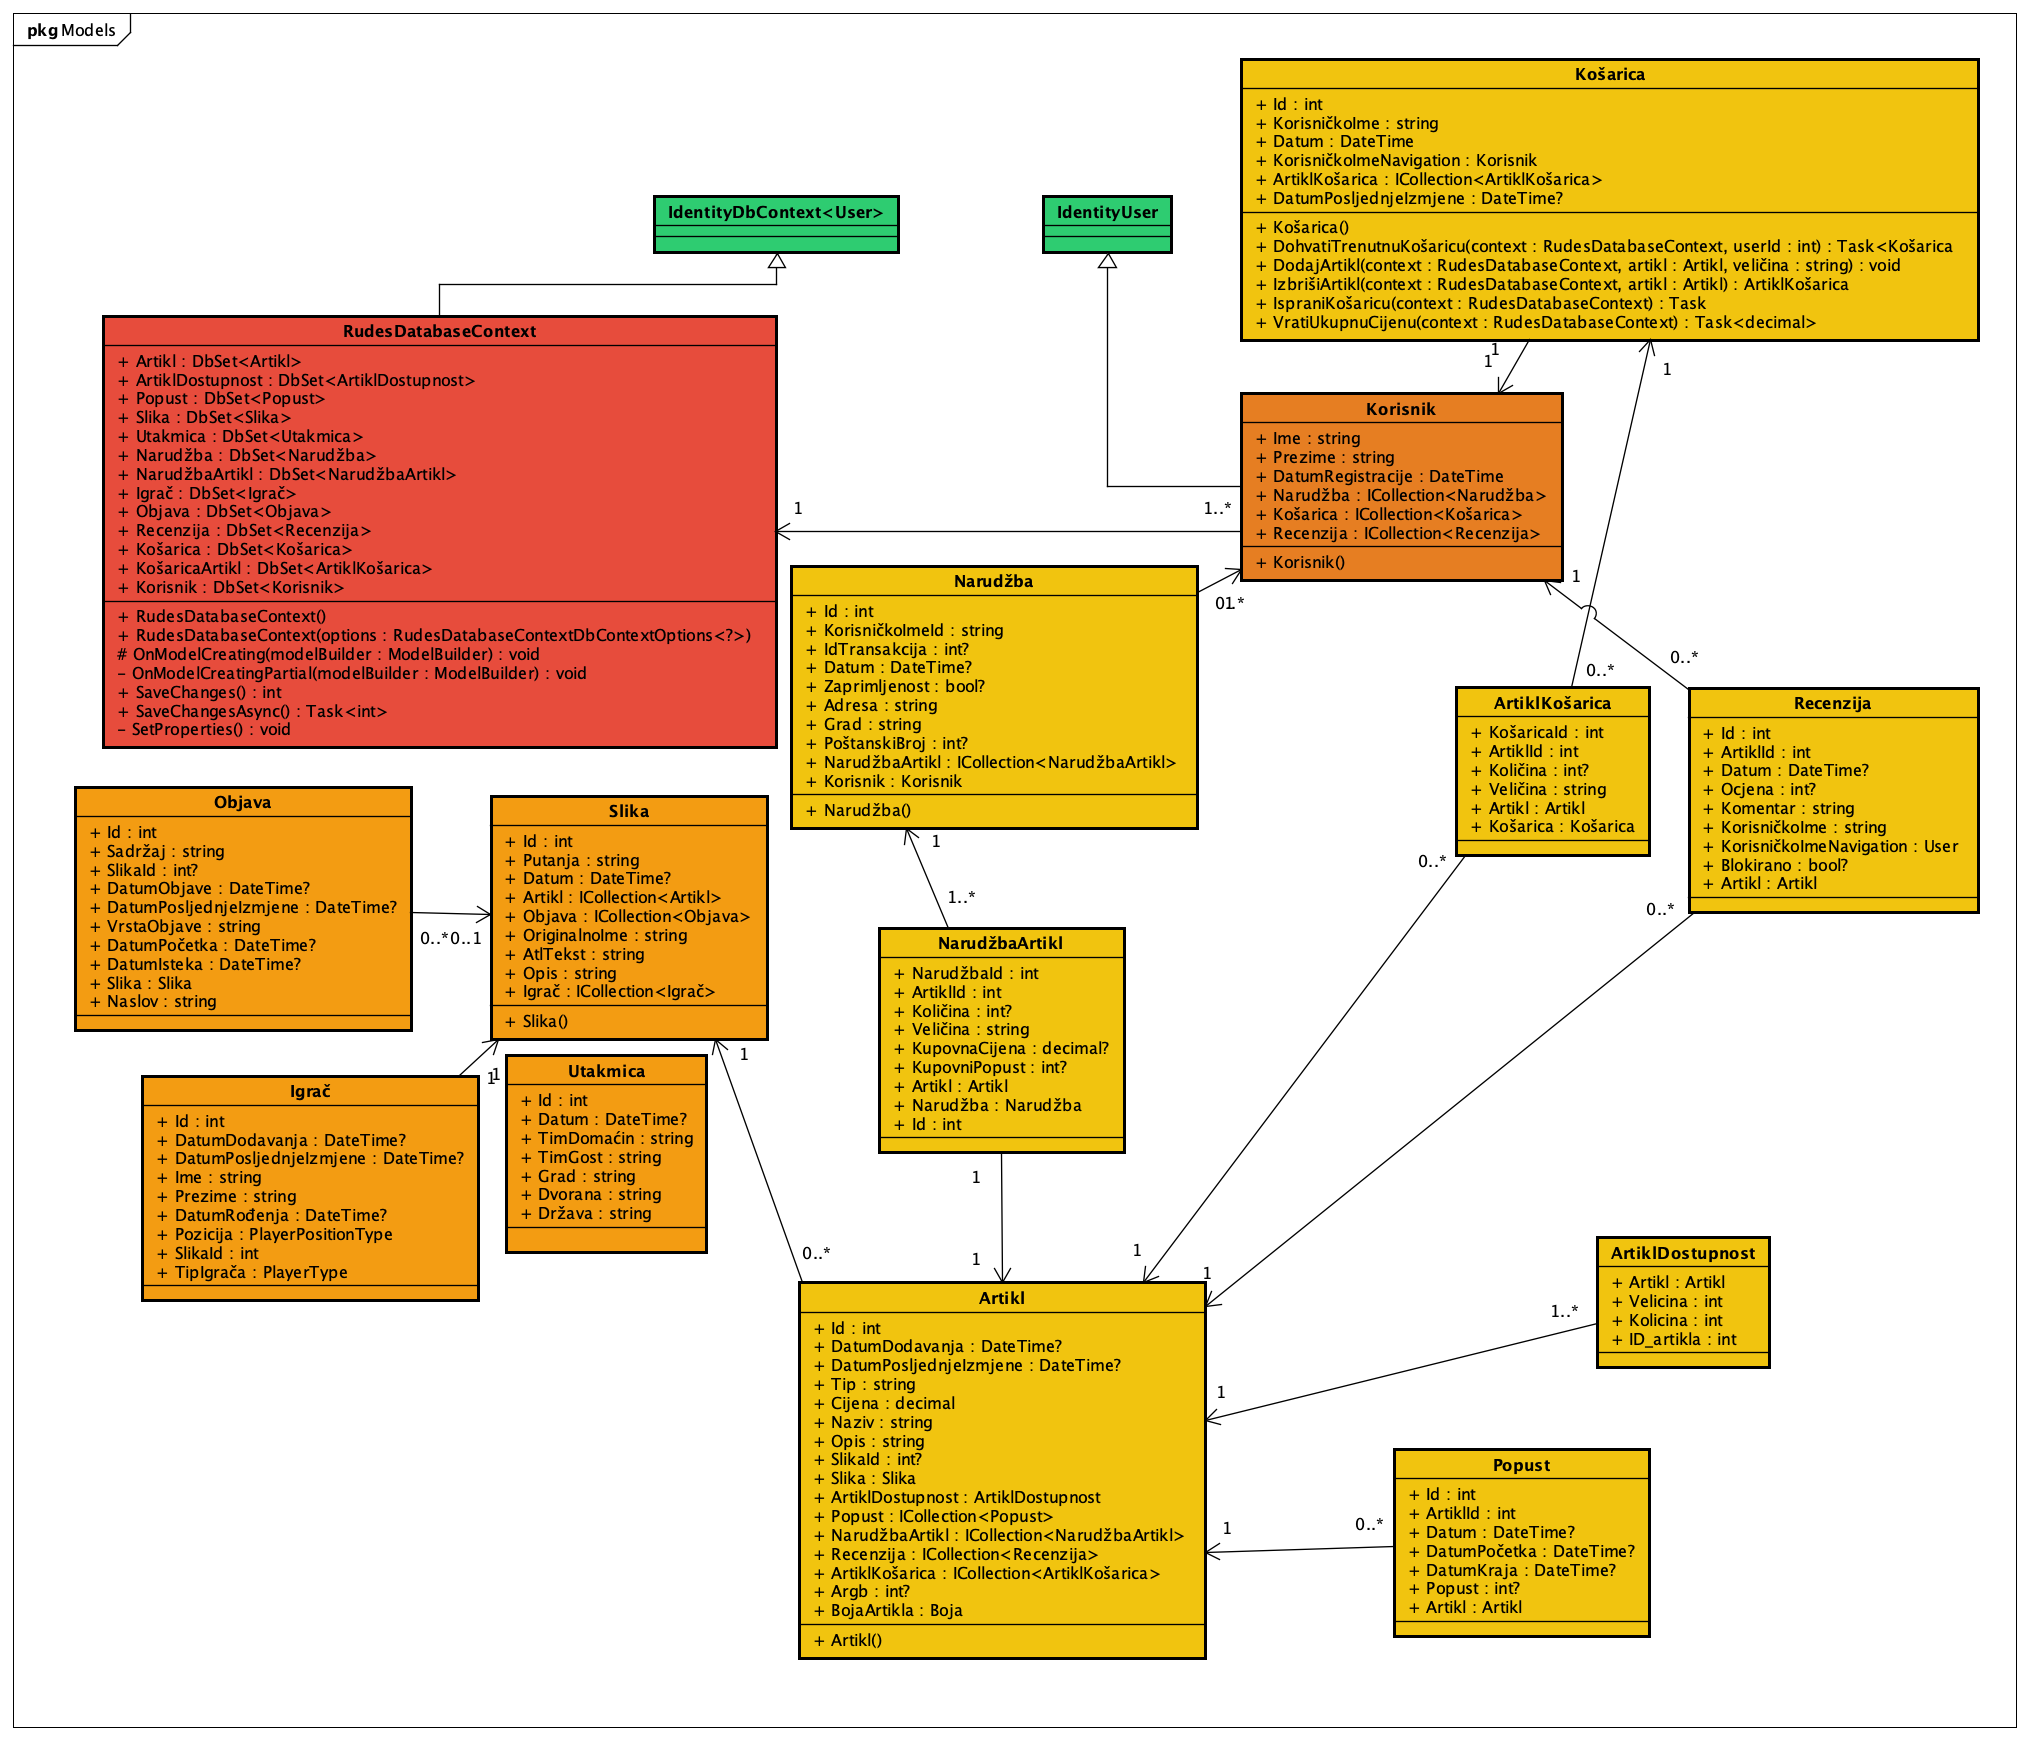
\includegraphics[width=\linewidth]{dijagrami/DijagramRazredaModels.png}
			\centering
			\caption{Dijagram razreda - dio Models}
			\label{fig:ClassDiagram1}
		\end{figure}
			
		%	\textbf{\textit{dio 1. revizije}}\\
			
		%	\textit{Prilikom prve predaje projekta, potrebno je priložiti potpuno razrađen dijagram razreda vezan uz \textbf{generičku funkcionalnost} sustava. Ostale funkcionalnosti trebaju biti idejno razrađene u dijagramu sa sljedećim komponentama: nazivi razreda, nazivi metoda i vrste pristupa metodama (npr. javni, zaštićeni), nazivi atributa razreda, veze i odnosi između razreda.}\\
			
		%	\textbf{\textit{dio 2. revizije}}\\			
			
		%	\textit{Prilikom druge predaje projekta dijagram razreda i opisi moraju odgovarati stvarnom stanju implementacije}
			
			
			
			\eject
		
		% \section{Dijagram stanja}
			
			
		% 	\textbf{\textit{dio 2. revizije}}\\
			
		% 	\textit{Potrebno je priložiti dijagram stanja i opisati ga. Dovoljan je jedan dijagram stanja koji prikazuje \textbf{značajan dio funkcionalnosti} sustava. Na primjer, stanja korisničkog sučelja i tijek korištenja neke ključne funkcionalnosti jesu značajan dio sustava, a registracija i prijava nisu. }
			
			
		% 	\eject 
		
		% \section{Dijagram aktivnosti}
			
		% 	\textbf{\textit{dio 2. revizije}}\\
			
		% 	 \textit{Potrebno je priložiti dijagram aktivnosti s pripadajućim opisom. Dijagram aktivnosti treba prikazivati značajan dio sustava.}
			
		% 	\eject
		% \section{Dijagram komponenti}
		
		% 	\textbf{\textit{dio 2. revizije}}\\
		
		% 	 \textit{Potrebno je priložiti dijagram komponenti s pripadajućim opisom. Dijagram komponenti treba prikazivati strukturu cijele aplikacije.}
	\chapter{Implementacija i korisničko sučelje}
		
		
		\section{Korištene tehnologije i alati}
			
			\textnormal{
			Timski rad na ovom projektu zahtjeva konstanto surađivanje i praćenje
			stupnja razvijenosti aplikacije u procesu razvoja. Stoga je kao sustav za praćenje razvoja aplikacije korišten git. Git se sastoji od udaljenog, zajedničkog repozitorija, pohranjenog na poslužitelju GitLab, i lokalnih repozitorija svakog timskog člana što osigurava kontinuirano praćenje napretka, te na taj način svi imaju uvid u najnovije stanje i promjene dokumentacije i izvornoga koda aplikacije.}
		
			\smallbreak
			
			\textnormal{
			Za izradu dokumentacije korišten je programski jezik LaTeX. Za
			razliku od ostalih poznatih uređivača teksta LaTeX dopušta surađivanje sustavom Git. Dokumentacija je pisana u uređivačkom programu TeXstudio, a odabrani prevoditelj je texLive. Dijagrami su napravljeni u uređivačkom programu Astah Professional, a u dokumentaciju su uvezeni kao .png slike generirane is Astah programa.}
		
			\smallbreak
			
			\textnormal{
			Za razvojno okruženje odabran je Microsoft Visual Studio, tvrtke
			Microsoft. Za radni okvir aplikacije odabran je ASP.NET Core koji podržava razvoj web aplikacija uključujući web servise, web resurse i web API-je. Razvojni model aplikacije je MVC (Model, View, Controller).
			Datoteke View komponente (frontend) su pisane u prezentacijskom jeziku HTML, stilskom jeziku CSS i skriptnom programskom jeziku JavaScript.
			Za kreiranje reaktivnih stranica (single-page applications, SPA) i korisničkih sučelja u frontendu korišten je Vue.js javascript okvir.
			Za pisanje datoteka u komponentama Model i Controller (backend) korišten je programski jezik C\#.
			Baza podataka se nalazi na poslužitelju u oblaku Microsoft Azure.\\
			\\
			\url{https://git-scm.com/}\\
			\url{https://gitlab.com/}\\
			\url{https://www.latex-project.org/}\\
			\url{http://astah.net/editions/professional}\\
			\url{https://visualstudio.microsoft.com/}\\
			\url{https://docs.microsoft.com/en-us/aspnet/core/?view=aspnetcore-3.1}\\
			\url{https://docs.microsoft.com/en-us/dotnet/csharp/}\\
			\url{https://www.javascript.com/}\\
			\url{https://portal.azure.com/}\\
			\url{https://vuejs.org/}}
			
			
			\eject 
		
	
		\section{Ispitivanje programskog rješenja}
			
			\textbf{\textit{dio 2. revizije}}\\
			
			 \textnormal{Popularni pristup razvoju testiranja (TDD) je pisanje testa prije implementacije ciljanog koda.  	Testiranje aplikacija postalo je uobičajena praksa za današnje softvere, a xUnit je jedan od najpopularnijih okvira za testiranje jedinica dostupan za .NET. Pisan je u jeziku C\#. U našoj aplikaciji smo također koristili xUnit te smo testiranja pisali po obrascima uporabe. Uvijek smo ponavljali isti pristup, pisali smo neuspjeli test i zatim ažurirali ciljni kod koji treba proći.Napisali smo 24 xUnit testa kako bismo testirali većinu naših obrazaca uporabe (za one jako jednostavne nisu ni bili potrebni testovi), no zbog jednostavnosti opisat ćemo samo tri integracijska testa.}
			 \bigbreak
			 \textnormal {	Prvi, jedan od najvažnijih testova, jest test prijave u sustav (UC3). Test prijave u sustav provjerava prijavu u svim ulogama: admin, trener, član uprave i kijent. Sastoji se od nekoliko funkcija u kojima se provjerava u bazi ispravnost korisničkog imena i lozinke. Na primjer, korisnik se ne može prijaviti s netočnom formom e-mail adrese. }
			 	\begin{packed_item}
			 	
			 	\item Prijava u sustav s e-mail adresom abc.com (pogrešna forma e-maila)
			 	\item[] \begin{packed_enum}
			 		\item očekivani ishod: aplikacija javi korisniku da e-mail nije dobro unesen e-mail i ne dozvoljava mu prijavu u sustav te nudi opciju da pokuša ponovno.
			 		\item očekivani ishod xUnit testa: test bi dao HTML odgovor da je prijava neuspjela
			 	\end{packed_enum}
			 \end{packed_item}
		 \textnormal {Ishod je bio kao što je i očekivano, odnosno test je prošao.}
		 
		 	\begin{packed_item}
		 	
		 	\item Prijava u sustav s netočnom lozinkom/e-mailom
		 	\item[] \begin{packed_enum}
		 		\item očekivani ishod: aplikacija javlja korisniku da mu je lozinka/mail pogrešan, odnosno da to nije važeći račun i onemogućava mu prijavu
		 		\item očekivani ishod xUnit testa: test vraća HTML odgovor o neuspjeloj prijavi
		 		
		 	\end{packed_enum}
		 \end{packed_item}
		 \textnormal {Ishod se i u ovom slučaju podudarao s očekivanim, odnosno test je ponovno prošao.}
		 \bigbreak
		 \textnormal {Drugi test koji ćemo spomenuti jest dohvaćanje postojećih objava. Test je osmišljen tako da korisnik mora biti ulogiran kao admin ili trener da bi mogao pristupiti objavama te provjerava za svaku pojedinačnu dohvaćenu objavu postoji li u bazi podataka te ako ne postoji, odnosno ako se prikazala pogrešna lista, vraća očekivanu poruku. Test je prošao.}
		 \bigbreak
		 \textnormal{Treći test je također vezan za objave, a može biti i za bilo koji dio baze podataka (slika, artikl, košarica). U tom se testu provjerava ispravno dohvaćanje, brisanje te traženje objave. Korisnik mora imati određenu razinu autorizacije, inače ne može tome pristupiti. Nakon što korisnik dohvati objavu, ako je dobro dohvaćena, može ju izbrisati i izbriše ju te joj pokuša ponovno pristupiti. Test bi trebao vraćati “Not found” status, odnosno ako baza ispravno radi, objava je iz nje izbrisana i ne može ju se dohvatiti. U ova se dva testa provjeravala ispravnost baze podataka. I ovaj je test prošao.
		 }
	
			
			\subsection{Ispitivanje komponenti}
			\textit{Potrebno je provesti ispitivanje jedinica (engl. unit testing) nad razredima koji implementiraju temeljne funkcionalnosti. Razraditi \textbf{minimalno 6 ispitnih slučajeva} u kojima će se ispitati redovni slučajevi, rubni uvjeti te izazivanje pogreške (engl. exception throwing). Poželjno je stvoriti i ispitni slučaj koji koristi funkcionalnosti koje nisu implementirane. Potrebno je priložiti izvorni kôd svih ispitnih slučajeva te prikaz rezultata izvođenja ispita u razvojnom okruženju (prolaz/pad ispita). }
			
			
			
			\subsection{Ispitivanje sustava}
			
			 \textit{Potrebno je provesti i opisati ispitivanje sustava koristeći radni okvir Selenium\footnote{\url{https://www.seleniumhq.org/}}. Razraditi \textbf{minimalno 4 ispitna slučaja} u kojima će se ispitati redovni slučajevi, rubni uvjeti te poziv funkcionalnosti koja nije implementirana/izaziva pogrešku kako bi se vidjelo na koji način sustav reagira kada nešto nije u potpunosti ostvareno. Ispitni slučaj se treba sastojati od ulaza (npr. korisničko ime i lozinka), očekivanog izlaza ili rezultata, koraka ispitivanja i dobivenog izlaza ili rezultata.\\ }
			 
			 \textit{Izradu ispitnih slučajeva pomoću radnog okvira Selenium moguće je provesti pomoću jednog od sljedeća dva alata:}
			 \begin{itemize}
			 	\item \textit{dodatak za preglednik \textbf{Selenium IDE} - snimanje korisnikovih akcija radi automatskog ponavljanja ispita	}
			 	\item \textit{\textbf{Selenium WebDriver} - podrška za pisanje ispita u jezicima Java, C\#, PHP koristeći posebno programsko sučelje.}
			 \end{itemize}
		 	\textit{Detalji o korištenju alata Selenium bit će prikazani na posebnom predavanju tijekom semestra.}
			
			\eject 
		
		
		\section{Dijagram razmještaja}
			
			\textbf{\textit{dio 2. revizije}}
			
			 \textit{Potrebno je umetnuti \textbf{specifikacijski} dijagram razmještaja i opisati ga. Moguće je umjesto specifikacijskog dijagrama razmještaja umetnuti dijagram razmještaja instanci, pod uvjetom da taj dijagram bolje opisuje neki važniji dio sustava.}
			
			\eject 
		
		\section{Upute za puštanje u pogon}
		
			\textbf{\textit{dio 2. revizije}}\\
			 
			 \textnormal{Aplikacija je razvijena u okviru ASP.NET Core 3 uz korištenje SQL Server relacijske baze podataka. Prilikom izrade baze podataka koristili smo pristup "Database First". To znači da smo prvo konstruirali bazu, izgenerirali SQL kod za nju te pomoću .NET Core-a izgenerirali C\# razrede koji opisuju strukturu baze. Kako bismo osigurali da se aplikacija može spojiti na bazu, potrebno je u datoteci "appsettings.json" podesiti connection string na vrijednost: "\textit{Server=(localdb)\\mssqllocaldb;Database=RudesDatabase;Trusted\_Connection=True;}". Prilikom prvog pokretanja aplikacije, potrebno je ispuniti bazu podacima iz seeder razreda, a to se radi pomoću linije "\textit{RudesDatabaseSeeder.Initialize(app);}" u datoteci Startup.cs. Nakon toga, dovoljno je aplikaciju pokrenuti odabirom "Run" pa "Start without Debugging".}
			 
			 \begin{figure}[H]
			 	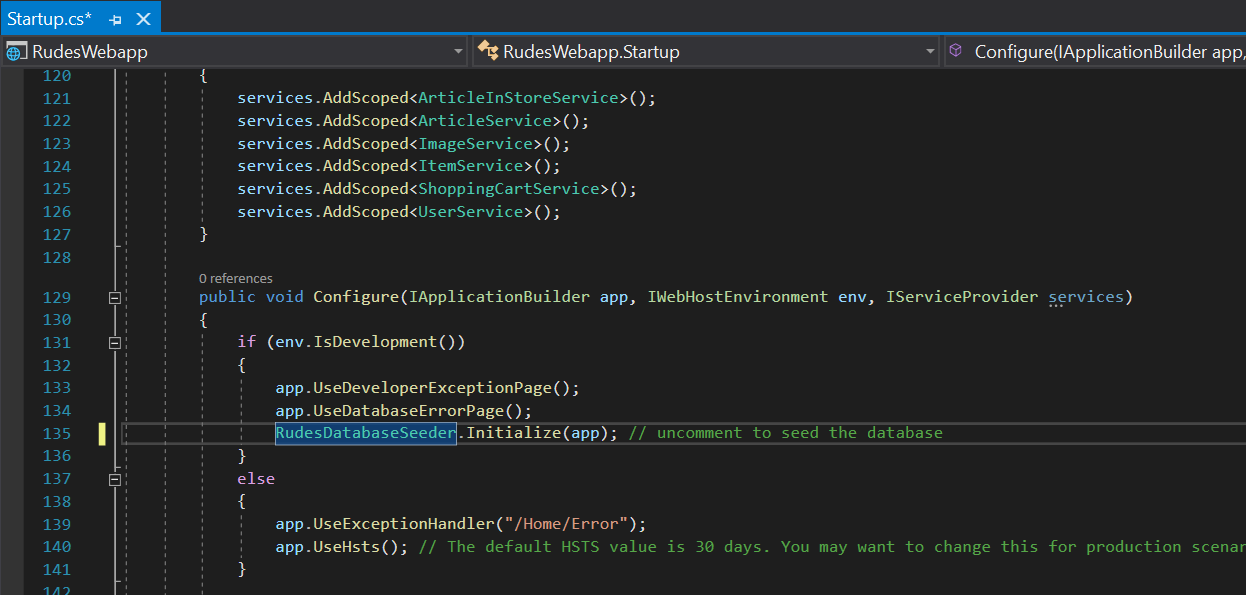
\includegraphics[width=\linewidth]{deployment/database_seeder.png}
			 	\centering
			 	\caption{Inicijalizacija Database Seeder-a}
			 	\label{fig:ClassDiagram1}
			 \end{figure}
			 
			 \textnormal{Ukoliko je došlo do promjena u bazi podataka, prije idućeg pokretanja aplikacije potrebno je u Package Manager Console pokrenuti naredbu "Update-Database" kako bi se ažurirale vrijednosti u tablicama baze. Nakon toga se aplikacija može ponovno pokrenuti.}
			 
			 \begin{figure}[H]
			 	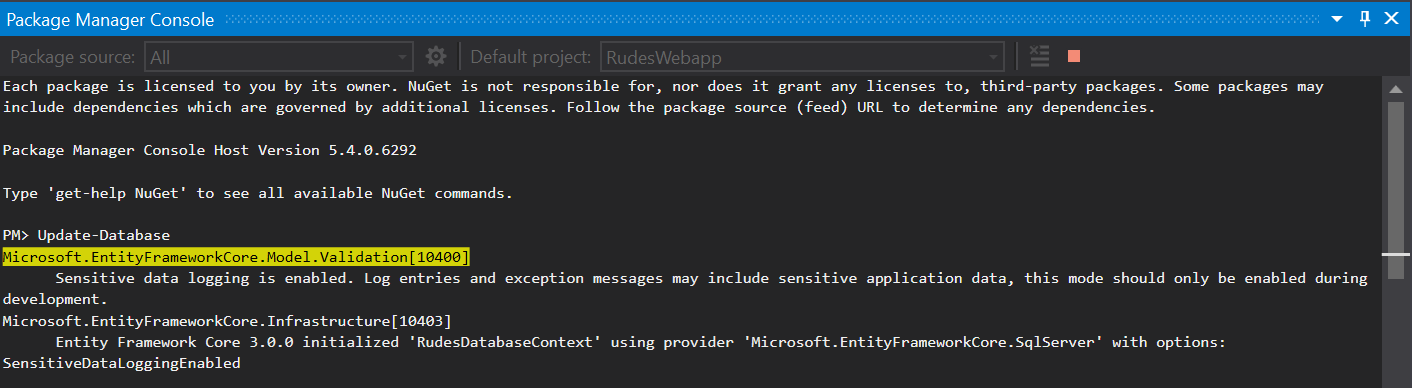
\includegraphics[width=\linewidth]{deployment/pmc_update_database.png}
			 	\centering
			 	\caption{Update-Database naredba u Package Manager Console}
			 	\label{fig:ClassDiagram1}
			 \end{figure}	
			
			\eject 
	\chapter{Zaključak i budući rad}
		
		\textbf{\textit{dio 2. revizije}}\\
		
		 \textit{U ovom poglavlju potrebno je napisati osvrt na vrijeme izrade projektnog zadatka, koji su tehnički izazovi prepoznati, jesu li riješeni ili kako bi mogli biti riješeni, koja su znanja stečena pri izradi projekta, koja bi znanja bila posebno potrebna za brže i kvalitetnije ostvarenje projekta i koje bi bile perspektive za nastavak rada u projektnoj grupi.}
		
		 \textit{Potrebno je točno popisati funkcionalnosti koje nisu implementirane u ostvarenoj aplikaciji.}
		
		\eject 
	\chapter*{Popis literature}
		\addcontentsline{toc}{chapter}{Popis literature}
	 	

		\begin{enumerate}
			
			
			\item  Oblikovanje programske potpore, FER ZEMRIS, \url{http://www.fer.hr/predmet/opp}
			
			\item  I. Sommerville, "Software engineering", 8th ed, Addison Wesley, 2007.
			
			
			\item  Astah Community, \url{http://astah.net/editions/uml-new}
			
			\item Holistics Software, \url{https://dbdiagram.io/home}
			
			\item ASP.NET Documentation,
			\url{https://docs.microsoft.com/en-us/aspnet/}
			
			\item Entity Framework Documentation,
			\url{https://docs.microsoft.com/en-us/ef/}
			
			\item Get started with Azure,
			\url{https://docs.microsoft.com/en-us/azure/}
			
			\item  Joseph Albahari, "C# 7.0 in a Nutshell: The Definitive Reference", 7th ed, , 2018.
			
			
		\end{enumerate}
		
		 
	
	
	\begingroup
	\renewcommand*\listfigurename{Indeks slika i dijagrama}
	%\renewcommand*\listtablename{Indeks tablica}
	%\let\clearpage\relax
	\listoffigures
	%\vspace{10mm}
	%\listoftables
	\endgroup
	\addcontentsline{toc}{chapter}{Indeks slika i dijagrama}


	
	\eject 
		
	\chapter*{Dodatak: Prikaz aktivnosti grupe}
		\addcontentsline{toc}{chapter}{Dodatak: Prikaz aktivnosti grupe}
		
		\section*{Dnevnik sastajanja}
		
		\begin{packed_enum}
			\item  sastanak
			
			\item[] \begin{packed_item}
				\item Datum: 4. listopada 2019.
				\item Prisustvovali: svi (7)
				\item Zapisnik piše: Frano Rajič
				\item Teme sastanka:
				\begin{packed_item}
					\item kratko upoznavanje tima
					\item dogovor oko korištenja Gita
					\item dogovor oko kanala komunikacije
					\item pregled rokova projekta
					\item razmatranje ponuđene teme projekta
					\item dogovor oko pisanja zapisnika
					\item dogovor sljedećih koraka
				\end{packed_item}
			\end{packed_item}
						
			\item  sastanak
			\item[] \begin{packed_item}
				\item Datum: 8. listopada 2019.
				\item Prisustvovali: svi (7)
				\item Zapisnik piše: Ana Šobot
				\item Teme sastanka:
				\begin{packed_item}
					\item detaljni pregled teme predložene pod imenom "IznajmiRomobil" 
					\item predstavljanje naših tema
					\begin{packed_item}
						\item "Duolingo"
						\item "KK Rudeš"
						\item "Kanal komunikacije za srednjoškolce"
					\end{packed_item}
					\item biranje između 4 teme
					\item dogovor oko korištenih tehnologija (ASP.NET CORE, C\#, HTML, CSS, JavaScript, Vue.js)
				\end{packed_item}
			\end{packed_item}

			\pagebreak

			\item  sastanak
			\item[] \begin{packed_item}
				\item Datum: 25. listopada 2019.
				\item Prisustvovali: svi (7)
				\item Zapisnik piše: Petar Bubica
				\item Teme sastanka:
				\begin{packed_item}
					\item pregled sadržaja dokumentacije
					\item podjela posla oko pisanja dokumentacije
					\item općenita podjela posla oko implementacije
					\item pregled korištenih grana u Gitu
				\end{packed_item}
			\end{packed_item}

			\item  sastanak
			\item[] \begin{packed_item}
				\item Datum: 2. studenoga 2019.
				\item Prisustvovali: svi (7)
				\item Zapisnik piše: Filip Todorić
				\item Teme sastanka:
				\begin{packed_item}
					\item dodavanje osnovnih dijelova frontenda
					\item dizajniranje baze podataka
				\end{packed_item}
			\end{packed_item}
			
			\item  sastanak
			\item[] \begin{packed_item}
				\item Datum: 5. studenoga 2019.
				\item Prisustvovali: svi (7)
				\item Zapisnik piše: Frano Rajič
				\item Teme sastanka:
				\begin{packed_item}
					\item frontend development
					\item podešavanje lokalne baze podataka
					\item database first pristup stvaranju modela
				\end{packed_item}
			\end{packed_item}
			
			\item  sastanak
			\item[] \begin{packed_item}
				\item Datum: 7. studenoga 2019.
				\item Prisustvovali: svi (7)
				\item Zapisnik piše: Frano Rajič
				\item Teme sastanka:
				\begin{packed_item}
					\item frontend development
					\item stvaranje razreda koji predstavljaju modele baze podataka
				\end{packed_item}
			\end{packed_item}
			
		\end{packed_enum}
		
		\eject
		\section*{Tablica aktivnosti}
		
			\textbf{\textit{Kontinuirano osvježavanje}}\\
			
			 \textit{Napomena: Doprinose u aktivnostima treba navesti u satima po članovima grupe po aktivnosti.}
					
			\begin{longtabu} to \textwidth {|X[7, l]|X[1, c]|X[1, c]|X[1, c]|X[1, c]|X[1, c]|X[1, c]|X[1, c]|}
								
				\cline{2-8} \multicolumn{1}{c|}{\textbf{}} &     \multicolumn{1}{c|}{\rotatebox{90}{\textbf{Frano Rajič }}} & \multicolumn{1}{c|}{\rotatebox{90}{\textbf{Petar Bubica }}} &	\multicolumn{1}{c|}{\rotatebox{90}{\textbf{Filip Todorić }}} &	\multicolumn{1}{c|}{\rotatebox{90}{\textbf{Dorotea Franjić }}} &
				\multicolumn{1}{c|}{\rotatebox{90}{\textbf{Ivan Skorupan }}} &
				\multicolumn{1}{c|}{\rotatebox{90}{\textbf{Danica Vladić }}} &	\multicolumn{1}{c|}{\rotatebox{90}{\textbf{Ana Šobot }}} \\ \hline 
				\endfirsthead
				
			
				\cline{2-8} \multicolumn{1}{c|}{\textbf{}} &     \multicolumn{1}{c|}{\rotatebox{90}{\textbf{Frano Rajič }}} & \multicolumn{1}{c|}{\rotatebox{90}{\textbf{Petar Bubica }}} &	\multicolumn{1}{c|}{\rotatebox{90}{\textbf{Filip Todorić }}} &
				\multicolumn{1}{c|}{\rotatebox{90}{\textbf{Dorotea Franjić }}} &	\multicolumn{1}{c|}{\rotatebox{90}{\textbf{Ivan Skorupan }}} &
				\multicolumn{1}{c|}{\rotatebox{90}{\textbf{Danica Vladić }}} &	\multicolumn{1}{c|}{\rotatebox{90}{\textbf{Ana Šobot }}} \\ \hline 
				\endhead
				
				
				\endfoot
							
				 
				\endlastfoot
				
				Upravljanje projektom 		&  &  &  &  &  &  & \\ \hline
				Opis projektnog zadatka 	&  &  &  &  &  &  & \\ \hline
				
				Funkcionalni zahtjevi       &  &  &  &  &  &  &  \\ \hline
				Opis pojedinih obrazaca 	&  &  &  &  &  &  &  \\ \hline
				Dijagram obrazaca 			&  &  &  &  &  &  &  \\ \hline
				Sekvencijski dijagrami 		&  &  &  &  &  &  &  \\ \hline
				Opis ostalih zahtjeva 		&  &  &  &  &  &  &  \\ \hline

				Arhitektura i dizajn sustava	 &  &  &  &  &  &  &  \\ \hline
				Baza podataka				&  &  &  &  &  &  &   \\ \hline
				Dijagram razreda 			&  &  &  &  &  &  &   \\ \hline
				Dijagram stanja				&  &  &  &  &  &  &  \\ \hline
				Dijagram aktivnosti 		&  &  &  &  &  &  &  \\ \hline
				Dijagram komponenti			&  &  &  &  &  &  &  \\ \hline
				Korištene tehnologije i alati 		&  &  &  &  &  &  &  \\ \hline
				Ispitivanje programskog rješenja 	&  &  &  &  &  &  &  \\ \hline
				Dijagram razmještaja			&  &  &  &  &  &  &  \\ \hline
				Upute za puštanje u pogon 		&  &  &  &  &  &  &  \\ \hline 
				Dnevnik sastajanja 			&  &  &  &  &  &  &  \\ \hline
				Zaključak i budući rad 		&  &  &  &  &  &  &  \\  \hline
				Popis literature 			&  &  &  &  &  &  &  \\  \hline
				&  &  &  &  &  &  &  \\ \hline \hline
				\textit{Dodatne stavke kako ste podijelili izradu aplikacije} 			&  &  &  &  &  &  &  \\ \hline
				\textit{npr. izrada početne stranice} 				&  &  &  &  &  &  &  \\ \hline 
				\textit{izrada baze podataka} 		 			&  &  &  &  &  &  & \\ \hline 
				\textit{spajanje s bazom podataka} 							&  &  &  &  &  &  &  \\ \hline
				\textit{back end} 							&  &  &  &  &  &  &  \\  \hline
				 							&  &  &  &  &  &  &\\  \hline
				
				
			\end{longtabu}
					
					
		\eject
		% \section*{Dijagrami pregleda promjena}
		
		% \textbf{\textit{dio 2. revizije}}\\
		
		% \textit{Prenijeti dijagram pregleda promjena nad datotekama projekta. Potrebno je na kraju projekta generirane grafove s gitlaba prenijeti u ovo poglavlje dokumentacije. Dijagrami za vlastiti projekt se mogu preuzeti s gitlab.com stranice, u izborniku Repository, pritiskom na stavku Contributors.}
		
	


\end{document}